\chapter{Traffic Light Data for Prediction}\label{ch:prediction}

% TODO: Paper IV

\section{Introduction}

The fact that road users do not know when the traffic lights will change leads to several well-known problems. First, the issue of unneeded stopping and idling at red lights unnecessarily increases energy expenditure and emissions. In addition, not knowing about the upcoming traffic light's switching behavior also has negative impacts on road safety. There is a so-called dilemma zone when approaching a traffic light, where it unexpectedly turns yellow, and one must decide whether to stop before the light \cite{zhang_yellow_2014, suzuki_new_2018}. Often, this can lead to running a red light, speeding, or misunderstandings between drivers, increasing the overall risk of accidents.

Here, improved communication between vehicles and infrastructure elements could reduce the risk of accidents and traffic inefficiency \cite{sun_optimal_2020}. Such collaborative awareness is critical in current Cooperative Intelligent Transport Systems (C-ITS) research. Predicting traffic lights and communicating this prediction to vehicles, establishing the C-ITS day-1 service GLOSA, is one integral part of a more extensive portfolio of potential measures \cite{mellegard_day_2020}. Nonetheless, it is essential to consider that traffic light prediction is not strictly limited to GLOSA-like systems and may also lay the foundation for other application scenarios. For example, with the emergence of Augmented Reality, also in bike contexts \cite{matviienko_bikear_2022, kosch_notibike_2022}, there may be many more application scenarios than we currently envision.

Despite these encouraging prospects, traffic light prediction is currently associated with multiple challenges. Despite the widespread use of countdown displays at traffic lights in various countries \cite{nygardhs_cyclists_2021}, integrating a mobile system to access and utilize the residual phase time directly from the traffic light's control unit presents a significant challenge. This process contrasts with the operation of countdown displays, which transfer phase time internally to a countdown controller \cite{islam_improved_2016}.

A mobile system working across multiple intersections requires an interoperable data source. Here, the option exists to obtain the control programs directly, but without the current internal program state \cite{zweck_traffic_2013}. Since traffic-adaptive signals may only decide a few seconds before the next cycle how long the green phase will be switched \cite{islam_improved_2016}, this method is restricted to fixed-time traffic light control programs that always switch in the same manner \cite{zweck_traffic_2013}. However, only 161 out of 1731 intersection nodes in Hamburg run a fixed-time program as of 2023\footnote{This information could be extracted from a traffic control inventory of the LSBG / IVS1 (as of June 22, 2023) provided on request, in addition to an inquiry to the Hamburg Senate: \url{https://www.buergerschaft-hh.de/parldok/dokument/72143/ampelschaltsysteme_gruene_welle.pdf}}.

Due to these issues, another method for traffic light prediction has been established to deploy traffic light assistance services in the field. Most GLOSA applications use the residual time provided by Signal Phase and Timing (SPaT) messages generated on the intersection controller level and transmitted to the vehicle \cite{wagner_spatmap_2023}. However, such messages may only sometimes be available at the given location -- sometimes, as in this work, the prediction of traffic lights has to be performed purely by observing the outside state \cite{protschky_extensive_2014, protschky_adaptive_2014}. This chapter will discuss the various methods for obtaining traffic light state information and evaluate the practical methods for cyclists.

One issue we will investigate in more detail is the traffic-adaptiveness of the switching programs. Traffic-adaptive adjustments of switching programs are intended to improve the traffic flow at an intersection but have adverse effects on predictability due to short-term green time adjustments \cite{schweiger_elisatm_2011, bodenheimer_enabling_2014}. This issue means that a prediction based on historical data may not always be accurate to the second. Furthermore, a challenge when deploying a prediction algorithm is that traffic light data may not always arrive complete or on time \cite{protschky_extensive_2014, protschky_adaptive_2014}, which is particularly problematic when the prediction needs to adapt quickly to a short-term change. Hence, error tolerance and robustness against missing information are also essential. If the prediction is unavailable or inaccurate, it can quickly lead to a loss of trust for the user or even become a safety risk.

The goals of this chapter are as follows. First, we will investigate potential real-time traffic light data sources and evaluate their practicality for cyclist applications. Afterward, we will review approaches that address traffic-adaptive timing in traffic light predictions. Combining learnings from both domains, we establish methods for a traffic-light prediction infrastructure for Hamburg. Based on a broad analysis of the adaptivity seen in the real-time data, we will study for how many intersections a prediction could be challenging. This study allows us to conclude the suitability of our chosen prediction method. Finally, we evaluate the prediction algorithm's accuracy, availability, and scalability over a long-term period.

\section{Related Work}

Two main focuses of related studies can be identified: overcoming issues in obtaining traffic light data and predicting traffic lights based on that data. For data acquisition, decentralized and centralized systems have been studied. Largely independent of these studies, multiple prediction methods that aim to improve prediction accuracy have been proposed. However, a holistic approach to traffic light prediction requires interleaving both perspectives. It must be considered that the prediction method is influenced by the technical constraints the data acquisition system imposes. Learnings from both domains must be joined to develop a state-of-the-art prediction system.

\subsection{Decentralized Systems}

In Europe, a large body of research and investments is currently flowing toward decentralized traffic light data systems, especially those based on Dedicated Short-Range Communication (DSRC). Road Side Units (RSUs) are deployed at intersections to operate these systems, sending standardized radio messages on the 5.9 GHz frequency band. These standardized C-ITS messages include SPaT messages, which vehicles can directly collect with a corresponding antenna (On Board Unit, OBU). A SPaT message contains the current switching state of a traffic light and a residual time until the next switch, making it an ideal data foundation for GLOSA applications \cite{ibrahim_estimating_2019}. Thus, many studies related to GLOSA utilize this data foundation \cite{schweiger_elisatm_2011, rakha_eco-driving_2011, rakha_aeris_2012, li_open_2012, suramardhana_driver-centric_2014, xu_bb_2015, bernais_design_2016, nguyen_efficient_2016, choudhury_integrated_2016, stahlmann_multi-hop_2017, stahlmann_exploring_2018, plianos_predictive_2018, zhang_green_2020, chen_developing_2022}.

SPaT messages are typically generated within the intersection controller level \cite{zweck_traffic_2013} and transmitted directly to an RSU without a centralized server system. However, such a system is typically not entirely decentralized. To calculate the residual time, there is the need for an additional prediction module, which may communicate with a cloud system in which a prediction algorithm is running \cite{strobl_c-its_2019, neuner_leitfaden_2020}. Due to the decentralized message transmission, however, a key advantage of this approach is that every vehicle equipped with a capable radio antenna has access to this data foundation. Thus, this approach is highly interoperable and attractive for manufacturers. The main per-unit cost factor to equip intersections with the necessary RSUs \cite{niebel_cost-benefit-based_2013}.

A current research problem with decentralized approaches is the limited over-the-air radio transmission distance, especially when foliage blocks the line of sight. Since the 5.9 GHz frequency band resides closer to visible light's wavelength than other network carriers, such as 3G and 4G, it does not penetrate well through obstacles. In response to this issue, the C-Roads project, a prominent initiative in Europe's C-ITS landscape, submitted a statement advocating for the supplementation of the 5.9 GHz band with lower-frequency bands \cite{bohm_radio_2017}.

With DSRC only, Stahlmann et al. (2017) \cite{stahlmann_multi-hop_2017} show that obstacles may reduce the transmission range to less than 150 meters. The drop in the transmission rate is not immediate but gradual, which is why a partial message loss must always be assumed with this method. Sharara et al. (2019) \cite{sharara_impact_2019} provide more insights into the relation between packet loss, a GLOSA system's activation distance, and the speed advisory's effectiveness. The authors show that partial message loss up to 90\% is not a significant problem unless the transmission distance is cut down too much, impacting the speed advisory system's activation distance and effectiveness. In a simulation with a specific green time of 25 seconds, red time of 40 seconds, and amber time of 5 seconds, Sharara et al. (2019) \cite{sharara_impact_2019} find that the transmission distance should be at least 850 meters for a 100\% success rate of traversing the green light, while 300 meters only resulted in 50\% -- 60\% of green passes depending on the message loss rate (90\% -- 10\%). Thus, with the transmission distance reported by Stahlmann et al. (2017) \cite{stahlmann_multi-hop_2017}, GLOSA applications may occasionally fall short of their potential benefit simply due to the transmission distance of the SPaT messages.

One explored solution to improve transmission range is an optimized RSU placement \cite{mehar_optimized_2015, massobrio_smart_2015, al-ezaly_optimal_2020}. Another option may be to adjust the transmission rate, which is reported in different ranges of 4 Hz \cite{stahlmann_multi-hop_2017} to 10 Hz in Hamburg \cite{stegen_ideas_2021}. The third option is inter-vehicle relaying of the messages to artificially expand the transmission range, as proposed by Stahlmann et al. (2017) \cite{stahlmann_multi-hop_2017}. Thus, a few practical solutions have already been presented to mitigate the limited transmission distance problem. For smartphone applications without direct access to an OBU, external antennas have been developed that can be connected via a USB cable \cite{kim_vulnerable_2017}. Additionally, manufacturers Bosch\footnote{\url{https://www.bosch-presse.de/pressportal/de/en/auto-cycling-and-tech-innovators-launch-coalition-for-cyclist-safety-based-on-v2x-deployments-259136.html}} and Canyon\footnote{\url{https://media-centre.canyon.com/en-INT/226588-canyon-plan-to-integrate-autotalks-v2x-technology-into-bicycles-to-help-reduce-accidents}} may introduce OBUs into their bike components soon, making this technology more accessible to cyclists.

One emerging alternative to 5.9 GHz radio is cellular V2X. This transmission technology utilizes an existing carrier medium such as 4G or 5G for the message transfer \cite{xia_field_2012, zweck_traffic_2013, bhattacharyya_assessing_2022}, distributing messages directly from an RSU (decentralized) \cite{bohm_radio_2017} or via cell towers (semi-decentralized) \cite{strobl_c-its_2019, jacob_ivs-kom_2020}. Although this carrier medium is interoperable on the application level (transmitting SPaT messages), there seem to be incompatibility issues on the network level \cite{bohm_radio_2017}. Thus, while DSRC is widely deployed on roads in Austria and Germany\footnote{\url{https://auto-talks.com/technology/dsrc-vs-c-v2x/}}, cellular V2X may replace DSRC in the future\footnote{\label{cloudflight-article}\url{https://www.cloudflight.io/en/blog/5g-killer-app-v2x-requires-the-transformation-the-automotive-industry/}}. Amid this uncertain state, C-ITS pilots \cite{strobl_c-its_2019} and OBU manufacturers \cite{jacob_ivs-kom_2020} develop multi-band solutions working with cellular V2X and DSRC in parallel.

Another issue is the unclear long-term compatibility of cellular V2X with smartphones. Although chipsets exist that enable LTE-V2X through the PC5 mode (direct device-to-device communication) and LTE-V2X/5G-V2X via cell towers\footnote{\url{https://5gaa.org/content/uploads/2021/11/5GAA_List_of_C_V2X_devices.pdf}}, these chipsets are manufactured mainly for automotive applications. The 5G Automotive Association, a proponent of cellular V2X encompassing automotive and chipset manufacturers, predicted LTE-V2X in 2017 to penetrate 80\% of new smartphones by 2027\footnote{\url{https://5gaa.org/content/uploads/2017/12/5GAA-Road-safety-FINAL2017-12-05.pdf}}. However, this prediction is based on an optimistic scenario in which smartphone manufacturers react to increasing demand for C-ITS applications induced by LTE-V2X deployments in cars. There is also the pessimistic scenario in which 0\% of smartphones will support this technology in the future. Currently, it is up for speculation which scenario is more likely, meaning that cellular V2X is not yet an established data source for smartphone-based GLOSA applications.

\subsection{Centralized Systems}

While DSRC and cellular V2X aim to provide a near-range network for C-ITS message communication, there is also the option for a traditional approach over the internet. With this approach, the traffic light data is collected at a centralized server infrastructure located near the traffic management center and redistributed over an internet endpoint \cite{zweck_traffic_2013, protschky_extensive_2014, protschky_adaptive_2014}. A centralized traffic light data infrastructure circumvents two challenges of decentralized approaches: limited transmission range and long-term compatibility with smartphones. However, it also shifts the responsibility of interoperability, data processing, and quality assurance toward the service consumer.

At Audi, Zweck et al. (2013) \cite{zweck_traffic_2013} established a data foundation for a GLOSA system that ingests traffic light data from three major cities. Correspondingly, three data adapters needed to be implemented: In Verona, the car manufacturer had access to SPaT messages generated on the intersection controller level. In Garmisch, intersection controllers were retrofitted with an additional SWARCO forecast module to obtain the necessary data, presumably SPaT messages. In Berlin, multiple traffic control centers were connected with various protocols, for which the specific transmission format is not further disclosed. The implemented data adapters were integrated into a centralized proprietary backend of Audi, making the corresponding traffic light information available to the company's vehicles via a mobile network connection to the internet. Unfortunately, the specific prediction methods and challenges related to traffic light prediction are not provided in detail. The lack of transparency constrains the insights derived from this study and the potential knowledge gained. While it is generally unclear where this system is currently in operation, the available information indicates that the system was introduced in the United States in 2016 and is currently utilized to facilitate Audi's GLOSA services in Düsseldorf \cite{neuner_leitfaden_2020}.

Many studies, whether decentralized or centralized, utilize the contained prediction in SPaT messages directly to generate the GLOSA service without needing an additional prediction system. In this way, these studies delegate the task of traffic light prediction to the infrastructure provider. However, some occasions may lead to the circumstance that the SPaT messages are not directly processable or available. The stability of the messages may also not be guaranteed at all times. As a result, an external prediction algorithm may be required that is not only scalable across multiple hundred intersection nodes but also robust to data outages. This show studies by Protschky et al. (2014) \cite{protschky_extensive_2014, protschky_adaptive_2014}. In this study conducted for BMW, the authors were confronted with a relatively suboptimal data foundation in Munich. Usually, the delays in traffic light messages are within a few seconds \cite{neuner_leitfaden_2020}. However, in Munich, the authors had to work with SPaT messages arriving 10 to 60 minutes late due to the city's traffic light data infrastructure at the time. This significant delay meant that the residual prediction contained in the SPaT messages would be far outdated once the backend obtained this information. Furthermore, the traffic light messages were also partially incomplete. Thus, the authors devised a way to generate a prediction themselves. 

Protschky et al. (2014) \cite{protschky_extensive_2014, protschky_adaptive_2014} approached the challenges as follows. By recording the long-term history of a traffic light's actuation, the authors could generate a separate prediction decoupled from the real-time data, circumventing the message delays. Each generated prediction would contain a timeline between predicted "red" and "green" states after a given reference time. Short-term losses and errors were statistically filtered out by incorporating a longer time frame of recorded traffic light states into the prediction algorithm. Due to its computational simplicity, their approach can be considered highly scalable. When detecting that the prediction would no longer correlate with the actual observed data to over 95\% accuracy, as required by BMW, the prediction was turned off for the affected traffic lights. As a result, the prediction availability would sometimes drop below 69\% while improving the overall trustworthiness of the existing predictions. The possible implications of this drop in availability on the users were not studied.

Compared to decentralized systems, centralized approaches to obtaining traffic light data are much more compatible with cyclist applications and are still utilized today by at least one large car manufacturer. However, an ongoing challenge is to overcome the data issues of these systems. Protschky et al. (2014) \cite{protschky_extensive_2014, protschky_adaptive_2014} present an appealing solution that also applies to the data constraints in this work, in which no SPaT messages, and thus, no residual time predictions, are available. Their approach only requires real-time information on traffic light colors and their cycle timing -- both are available in Hamburg through the centralized platform that will present the foundation for our work. Potential improvements of this solution include a more focused study of the data characteristics, the suitability of the chosen prediction algorithm, and the user's perspective. One particular issue is the reduced prediction availability in the presence of traffic-adaptive signal timing.

\subsection{Traffic-Adaptive Signal Timing}

The accuracy of predictions is negatively affected by shifted switching behavior due to traffic-adaptive signal timing intended to optimize the traffic flow. As noted by Otto et al. (2023) \cite{otto_framework_2023}, the dynamic shifting of traffic light timing reduces the effectivity and trustworthiness of the speed advisory. However, whether the prediction is affected highly depends on the prediction algorithm. In general, there are two different approaches to prediction: self-adaptive and probabilistic prediction methods. Both respond differently to dynamics in traffic light behavior. Otto et al. (2023) \cite{otto_framework_2023} only refer to the traditional, probabilistic methods.

\begin{figure}[t]
\centering 
\begin{tabular}{ccc}
\footnotesize{(a) Fixed-time} & \footnotesize{(b) Partially adaptive} & \footnotesize{(c) Fully adaptive} \\
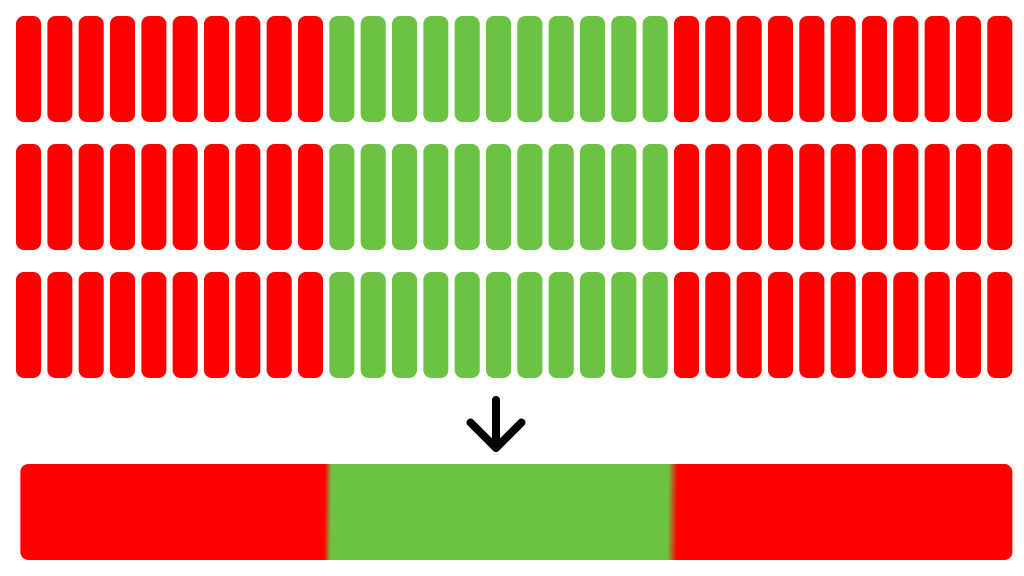
\includegraphics[width=0.3\linewidth]{images/explanation-fixed-time.png} & 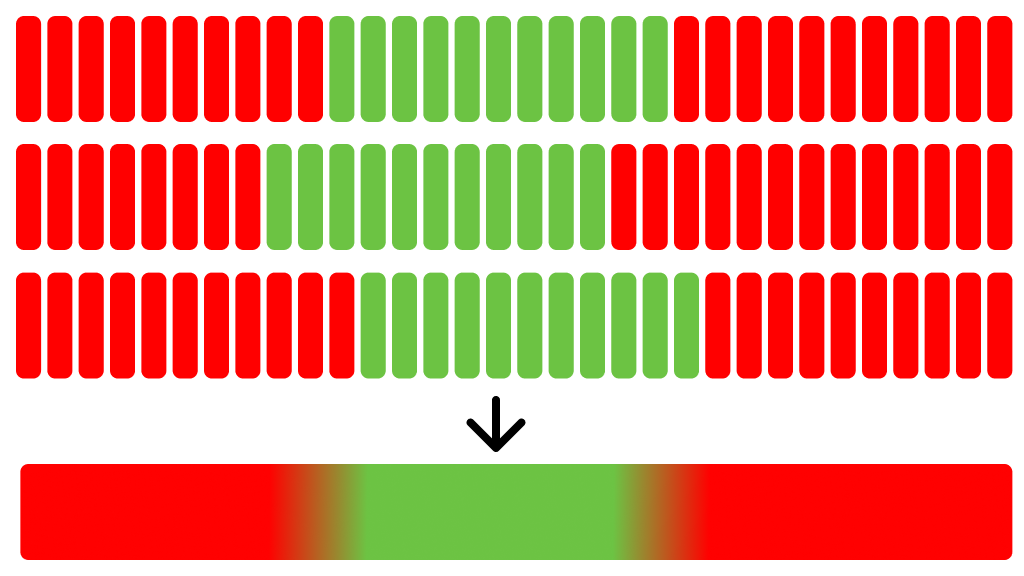
\includegraphics[width=0.3\linewidth]{images/explanation-partially-adaptive.png} & 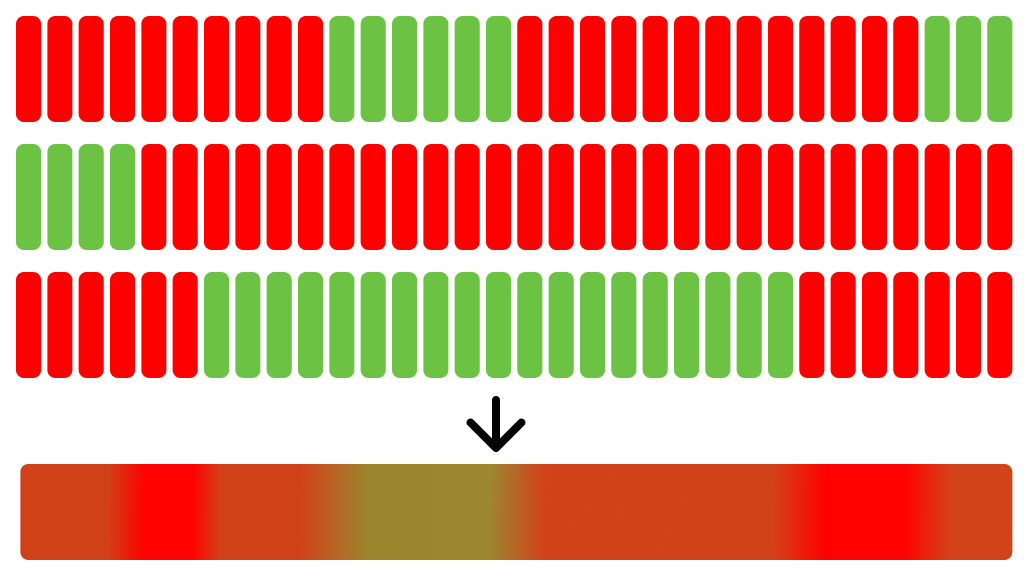
\includegraphics[width=0.3\linewidth]{images/explanation-fully-adaptive.png}
\end{tabular}
\caption{Probabilistic (cycle-stacking) method for prediction and its reaction to traffic-adaptive switching.}
\label{fig:prediction}
\end{figure}

A probabilistic method has been proposed by Protschky et al. (2014) \cite{protschky_extensive_2014, protschky_adaptive_2014}. The idea of this method is as follows. Since a fixed per-traffic-light cycle length is mandatory even with fully adaptive traffic light programs \cite{protschky_extensive_2014}, the recorded history can be convolved into a stack of cycles as highlighted in \Cref{fig:prediction}. Then, the probability of "green" and "red" is determined for each second through the prevalence of the predicted color at this specific second in previous cycles.

As discussed earlier, Protschky et al. (2014) \cite{protschky_extensive_2014, protschky_adaptive_2014} have shown that this method is not only scalable but also works well in the presence of high latencies or data losses of real-time traffic light messages. Since the adaptive component is represented as a probability, the speed advisory can focus on certain parts of the prediction, counteracting the adaptive behavior. This kind of prediction algorithm reacts to traffic adaptive signal timing by blurring out certain parts of the prediction. 

Thus, as discussed by Otto et al. (2023) \cite{otto_framework_2023}, with a highly adaptive traffic light, one challenge is that the green and red predicted phases can become indistinguishable. If a target speed is calculated, the speed advisory algorithm must decide which prediction parts are considered safe enough. No speed advisory can be calculated if no parts of the prediction exceed the defined certainty threshold. This is shown by Mahler et al. (2012) \cite{mahler_reducing_2012}, who developed an optimization method for calculating the optimal speed with an uncertain prediction. A recent work by Typaldos et al. (2023) \cite{typaldos_modified_2023} has further developed the idea of calculating a probabilistic/stochastic speed advisory. One challenge of this approach is that, as adaptability increases, it tends to converge more towards the midpoint of the green phase. Following the speed recommendation may result in the vehicle not reaching the traffic light precisely on time but instead with some delay.

Self-adaptive prediction models address this issue very differently. By continually adapting the prediction to the observed real-time state, the prediction gets more accurate as it approaches the actual switching time. Bodenheimer et al. (2014 -- 2015) \cite{bodenheimer_enabling_2014, bodenheimer_glosa_2015} were the first to propose such an approach through a graph-based method. This method observes the ingress directions at an intersection node and reconstructs the relation between the clearance timing of each direction. Schneegans et al. (2023) \cite{schneegans_prediction_2023} also demonstrate the possibility of utilizing Machine Learning models for this process. Here, the idea is to utilize a sequence prediction model trained on prerecorded timing data from a specific traffic light. Both models have the advantage that the predicted residual time readjusts toward the actual observed data at the expense of stretching or shortening the predicted residual time.

As Stahlmann et al. (2018) \cite{stahlmann_exploring_2018} point out, this stretching and shortening can also be seen as a significant disadvantage of this approach. Since repeated adjustments to the prediction during the intersection approach negatively impact usability, there is a clear tradeoff between the prediction's accuracy and temporal stability. The increased computational complexity of the presented Machine Learning models is also a factor that may negatively impact the prediction algorithm's scalability toward multiple thousand signals. There is currently no evidence supporting the scalability on a large scale as opposed to probabilistic approaches \cite{protschky_extensive_2014, protschky_adaptive_2014}. 

Furthermore, while the probabilistic approach is intrinsically robust to incomplete data and can drop individual cycles, error robustness is another factor to consider in evaluating self-adaptive models. These challenges must be addressed to employ such a model in practice. Most importantly, however, the traffic light data must arrive in time for the self-adaption to happen. Thus, self-adaptive prediction methods can only be employed when the traffic light data arrives with a low latency. In a situation such as reported by Protschky et al. (2014) \cite{protschky_extensive_2014, protschky_adaptive_2014} where traffic light messages may arrive with a delay of over 10 minutes, such models are likely not a good option.

To further address the dispute between probabilistic and self-adaptive methods, an overarching question is how many traffic lights are, in fact, traffic-adaptive and how much this impacts predictability. This question must be answered to determine the likelihood that users will encounter inaccurate predictions at intersections. 

In related work, various studies report different levels of adaptiveness. Cai et al. (2009) \cite{cai_adaptive_2009} were the first to report that "most" signals in their context are traffic-adaptive. Concrete numbers were presented by Bodenheimer et al. (2014)\footnote{Notably, the reported proportions of adaptive traffic lights are often not verifiable through external sources. For example, in the work by Bodenheimer et al. (2014) \cite{bodenheimer_enabling_2014}, which mentions 95\% adaptive traffic lights in Hamburg, it was only clarified upon inquiry that these results were based on a survey conducted by a service provider on behalf of Audi.} \cite{bodenheimer_enabling_2014}, who reported that 95\% of traffic lights in Hamburg were adaptive and 73\% in the ten largest German cities. Fakler et al. (2014) \cite{fakler_structures_2014} also found a high proportion of traffic-actuated control systems in German cities with over 50,000 inhabitants. Schneegans et al. (2022) \cite{scheegans_exploiting_2022} and Heckmann et al. (2023) \cite{heckmann_stage_2023} further support the conclusion that most traffic lights are operated by traffic-adaptive controls. Hao et al. (2019) \cite{hao_eco-approach_2019} noted the widespread deployment of actuated traffic light controllers in the US, while Avatefipour and Sadry (2019) \cite{avatefipour_traffic_2018} found that fixed timing is more prevalent in Malaysia. Grumert and Pereira (2022) \cite{grumert_heads-up_2022} observed that 70\% of traffic lights in Sweden are adaptive. However, there are also contradictory statements, such as Olaverri-Monreal et al. (2018) \cite{olaverri-monreal_implementation_2018} reporting that adaptive timing is only implemented in a small number of road networks, and the majority of urban areas still use pre-timed control systems.

Overall, most studies indicate that Germany predominantly utilizes traffic-adaptive signals, with findings in Hamburg roughly aligning with our analysis that counted 90.7\% (1570 out of 1731) adaptivity-capable traffic lights. However, the implications for predictability remain largely unexplored. While the capacity to adapt to traffic may exist, it might be underutilized or manifested only in minor adjustments, potentially resulting in a less significant impact on prediction accuracy, as indicated by the reported percentages. Presently, no study examines the real-world effects of adaptiveness on predictability.

\begin{Summary}[Summary of Research Gap]
While many works focus on decentralized data transmission, a centralized approach is currently the best option for cyclist applications. Most centralized platforms appear to retransmit SPaT messages generated at the intersection controller level. Here, the residual time prediction in SPaT messages can be directly used for a speed advisory application. However, in some cases, SPaT messages may not be available or arrive too late. An external prediction service that copes with data latencies or errors is necessary in these cases. Large-scale deployments of GLOSA must incorporate these concerns, meaning that not all proposed prediction methods may be practical.

A probabilistic prediction method is promising for implementing traffic light prediction. This approach has already proven effective in the context of centralized systems, as opposed to self-adaptive prediction methods. Whether self-adaptive models can contribute to an enhanced traffic light prediction is subject to data issues and the tradeoff between temporal stability and prediction accuracy. The temporal stability, i.e., how often the prediction is adapted to be accurate, also determines the usability and trustworthiness of the speed advisory. This factor also depends on the spontaneity of the traffic light switching behavior induced by traffic-adaptiveness.

Against this backdrop, while some studies pose traffic-adaptive switching behavior as their central motivation to develop more advanced prediction methods, it is unclear how justified these motivations are. Reported numbers of adaptive traffic lights provide a rough estimate but no definite conclusion about the actual predictability of traffic lights. Here, a direct analysis of traffic light data could help determine how many traffic lights exhibit adaptive behavior and how much this behavior impacts predictability. If adaptiveness is seen but is limited to a few seconds, it may necessitate reevaluation of developed prediction algorithms.
\end{Summary}

\section{Concept}\label{sec:signal-prediction}

We will conduct two steps to address the described research gaps. First, we will design a prediction infrastructure with the available data foundations in Hamburg, contributing to understanding real-world deployment challenges. Specifically, we will focus on the chain of information from the traffic lights to the cyclist and identify issues in the data transmission that require further consideration. 

Since our data infrastructure will also be bound to delays and losses in the traffic light messages, we have to find a prediction method designed to be robust against these issues while being extensible to other cities and highly scalable. The plan is to reuse the field-tested probabilistic prediction incorporating the desired capabilities. However, we must establish a robust data infrastructure around the prediction algorithm that provides the foundation for our mobile application. Based on the implemented data infrastructure and prediction algorithm, we collect long-term operational insights into the data quality and prediction of traffic lights in Hamburg, contributing to the overall understanding of the practical challenges of deploying a large-scale GLOSA system.

Finally, we address the need for more research on traffic light adaptiveness and predictability. We analyze how suitable the prediction algorithm is for our scenario based on the large-scale evaluation of our traffic light data. We design and evaluate two novel metrics that allow us to measure and systematize types of unpredictability in traffic lights. Based on these concepts, the goal is to develop a functional prediction infrastructure and learn more about traffic light prediction facets in a large-scale urban environment, thus addressing the identified research gaps.

\subsection{Data Infrastructure for Prediction Algorithm}

\begin{figure}[t]
\centering
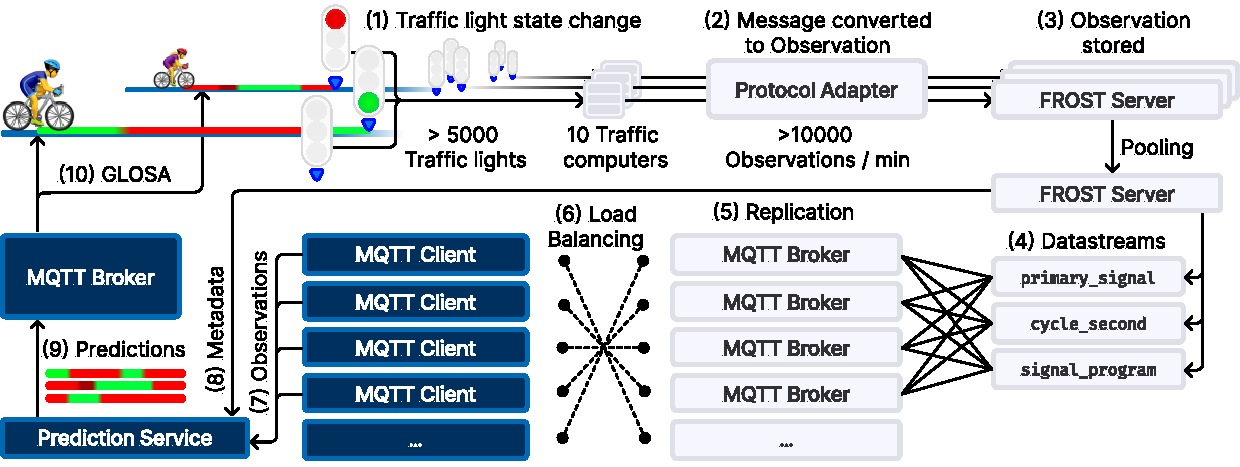
\includegraphics[width=\linewidth]{images/traffic-light-data-infrastructure.pdf}
\caption{Designed traffic light data adapter for Hamburg's Traffic Lights Data platform.}
\label{fig:traffic-light-data-infrastructure}
\end{figure}

To bring forward intelligent transport solutions such as GLOSA applications, Hamburg employs an open data policy through its self-imposed transparency law (HmbTG\footnote{\url{https://transparenz.hamburg.de/gesetzestext-des-hmbtg-636070}}), providing several kinds of urban data free of charge to the public. Hamburg provides static, continuously updated, real-time datasets and geo APIs as part of this urban data platform. One of these APIs is the Traffic Lights Data\footnote{\url{https://metaver.de/trefferanzeige?docuuid=AB32CF78-389A-4579-9C5E-867EF31CA225}} system, which provides real-time information about the switching of traffic lights in Hamburg and georeferences their location in the city. Published by the Free and Hanseatic City of Hamburg, Landesbetrieb Straßen, Brücken und Gewässer (LSBG), the data is made available under the DL-DE BY-2.0\footnote{\url{https://www.govdata.de/dl-de/by-2-0}} license and will be considered the foundation of this work.

One challenge of using the Traffic Lights Data platform for prediction and speed advisory in a GLOSA application is that the state messages are not provided in the SPaT format. Thus, no residual time prediction, as contained in SPaT messages, is available, meaning that an external prediction service is required to establish our GLOSA service. Changes in each traffic light's state are provided as real-time observations through the SensorThings\footnote{\url{https://www.ogc.org/standard/sensorthings/}} "Observation" format. Besides vehicle detector or bus request messages, three particular types of messages are essential for our prediction service:

\begin{itemize}
    \item \textbf{(Primary) signal color}: the current traffic light color and the time when this color was switched. Among green, red, amber, and amber-red, there are also other specific states such as amber-flashing, green-flashing, or dark (light turned off). The color is given for the primary signal head and supplementary signals, such as green arrows.
    \item \textbf{Signal program}: the current program ID running on the traffic light, with a timestamp when this program was switched.
    \item \textbf{Cycle second}: a timestamp indicating that program recirculation has happened. With this timing information, the continuous stream of colors can be split into cycles, usually 90, 75, or 60 seconds long. This information is also given for traffic lights that do not strictly use a circulating program routine.
\end{itemize}

The Traffic Lights Data platform was designed based on an existing traffic controller infrastructure and implemented by various stakeholders. The system design of the platform follows these technical and organizational constraints, resulting in a rather complex chain of information. As we will later see, precisely understanding this chain of information is crucial to tracing data issues that may arise. Thus, through dialogues with various Hamburg authorities, we reconstructed a precise picture of the infrastructure and potential points of failure.

To provide these messages in the Traffic Lights Data platform, they are translated and shifted multiple times between various data brokers. First, as seen in \Cref{fig:traffic-light-data-infrastructure}, the state messages are sent in a controller-specific format to one of ten traffic controllers (1). Then, the messages are converted to Observations (2) and sent to a corresponding SensorThings server. From there, a centralized SensorThings server collects all Observations (3), which are associated with a specific type of "Datastream" encapsulating the type of Observation: \texttt{primary\_signal} (color), \texttt{cycle\_second}, and \texttt{signal\_program} (4). Finally, the messages are published across an autoscaled Kubernetes cluster of MQTT brokers (5). 

From there, our prediction service connects to the broker endpoint to ingest all Observation messages. Our prediction service utilizes multiple MQTT clients with individual TCP connections to balance the load on each MQTT broker in the Traffic Lights Data platform (6). The collected Observations (7) are combined, knowing which Observation is associated with which Datastream of which traffic light through metadata in the Traffic Lights Data platform (8). This metadata allows the prediction service to record a history of program cycles and associate it with the corresponding traffic light ID. Based on these histories that are continuously updated, the probabilistic prediction method is executed periodically to keep predictions synced (9). 

The prediction algorithm itself was implemented by Sebastian Pape based on the method developed in his Diploma thesis \cite{pape_untersuchung_2012} and integrated into the data pipeline with corresponding programming interfaces. The programming interface converts the Observations into an internal format for the prediction algorithm, meaning that the programming interface is interoperable with other message formats as long as the three described types of traffic light state messages are given. Based on this foundation, the developed service could be seamlessly ported to other cities that provide the desired messages.

At its foundation, the integrated prediction method reconstructs cycles based on the cycle timing information and calculates which color will most likely appear for each second. To allow the prediction algorithm to adapt to changing programs, only the last ten cycles are kept for prediction. Then, every 60 seconds, the current history of each traffic light is fetched, and a new prediction is calculated based on the current time. The prediction is extrapolated over the regular cycle length to be 180 seconds long. This extrapolation will allow our app to display an appropriate speed advisory even when users are far from the traffic light. The generated prediction is published on an MQTT broker under the traffic light's ID, where the app is subscribed and automatically obtains new information. The prediction MQTT broker is configured to retain all messages, meaning that a new app subscription directly sends the last prediction for the subscribed traffic light. Finally, the app utilizes the obtained prediction to display a speed advisory.

\begin{figure}[t]
\centering
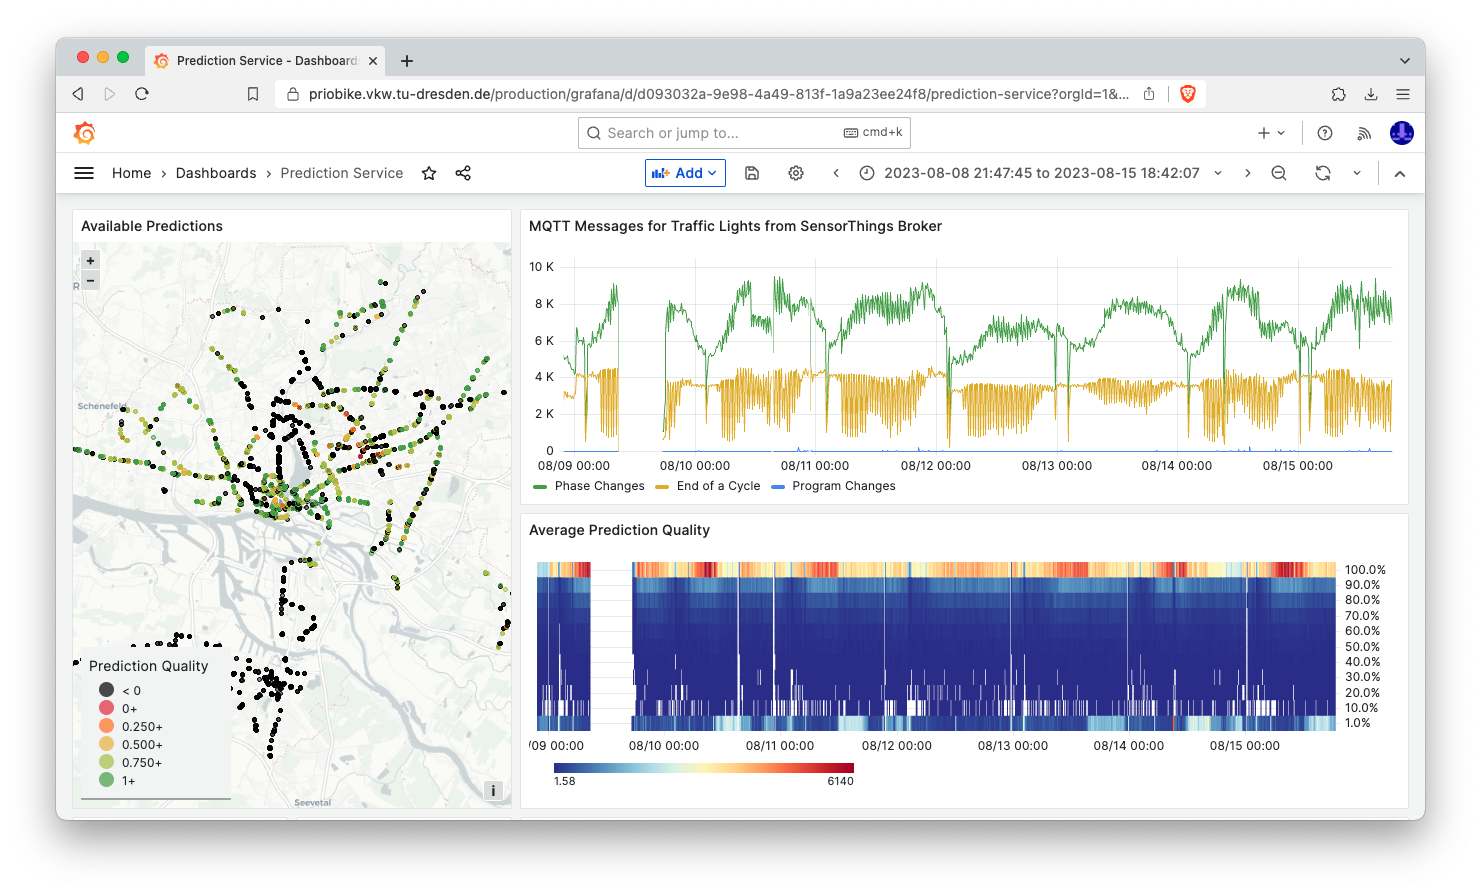
\includegraphics[width=\linewidth]{images/monitoring-screenshot.png}
\caption{Screenshot of the developed monitoring solution. [\hyperref[attribution]{Attribution}]}
\label{fig:monitoring-screenshot}
\end{figure}

A monitoring solution was developed to supervise whether the data infrastructure and the prediction algorithm work as intended. This solution, shown in \Cref{fig:monitoring-screenshot}, is based on a web dashboard that highlights real-time metrics such as the number of Observations, generated predictions, and spatial distribution of the measured prediction qualities. 

We also measure the number of invalid cycles, referring to cycles that contain invalid transitions between traffic light phases. Specifically, we check if a recorded cycle deviates from the regular switching patterns red--red-amber--green--amber and red--green. We check the length of amber against its maximum duration of 6 seconds, together with the maximum red-amber duration of 2 seconds, as specified by German traffic light operation constraints. Detected erroneous cycles are then discarded by the prediction service and logged by the monitoring system to identify outbreaks of erroneous data.

We can identify and report data failures to the platform operators based on discarded erroneous cycles, drops in the number of Observation messages, or a decreased prediction quality. Error patterns in the dropped messages allow us to provide more detailed information about the potential origins of data failures within the system's architecture.

For example, by viewing the prediction quality on a map, we can directly identify whether an outage is related to a specific traffic controller or associated with the complete city. If all city districts are affected, the problem is more likely to originate from the data pooling or load balancing components further along the information chain. Furthermore, we can study the time and duration of error patterns, giving us and the system's operators more clues about where to look for data issues. 

Finally, we deployed one additional monitoring instance at an external cloud provider to cross out issues from our TU Dresden deployment. Which error patterns could be identified and how the long-term data quality evolved will be discussed in the Results section of this chapter.

\subsection{Predictability Metrics}

Apart from dropped or delayed traffic light data, another aspect that influences the prediction quality is how unpredictably a traffic light switches. According to previous studies, generating a reliable forecast for traffic-adaptive signals could be challenging overall, especially in Hamburg. However, as we have seen in our literature study, direct predictability measurements have not been conducted so far. 

Since we had already established a method to obtain traffic light data from thousands of traffic lights in Hamburg, we identified a significant potential knowledge gain in conducting such a study. However, one key challenge is finding metrics that give us generalizable insights into predictability without being strictly bound to one prediction method. The idea is to measure how many predictable patterns are present or absent in the recorded data streams, i.e., how much the traffic light follows a predictable rhythm. The question is how to measure such a rhythm, as patterns could take various arrangements.

Until we arrived at our final metrics, we investigated various methods from other disciplines to measure if patterns are present in the switching behavior. For example, one idea was to measure the Shannon entropy of the traffic light's data stream, indicating how much information content and, thus, complexity of the switching behavior is present. Similarly, we attempted to use compression techniques to find how much information the present traffic light program could be compressed. Another idea was to utilize a fast Fourier transform to find how many different frequencies in the switching patterns were present, mapping a signal between green (1) and red (0). However, in the end, none of the attempted methods yielded a satisfactory measurement of how many predictable patterns were present while comparing the calculated values against case studies. 

Directly measuring the absence or presence of predictable patterns, agnostic from their concrete arrangement, was challenging based on the methods we considered. As an alternative, we found two more straightforward metrics that each capture critical unpredictability and can be used in conjunction.

The first kind of unpredictability we measure is the cycle discrepancy. This metric is calculated by counting different seconds between two cycles $C_1$ and $C_2$ with the length $l_1$ and $l_2$ in the recorded history:

\begin{equation} \text{Cycle Discrepancy}(C_1, C_2) =  \sum_{i=0}^{\max(l_1, l_2)-1} \left\{
\begin{array}{ll}
1 & \text{if } i \geq l_1 \text{ or } i \geq l_2 \\
1 & \text{if } C_1[i] \neq C_2[i] \\
0 & \text{otherwise}
\end{array} \right.\end{equation}

The cycle discrepancy is zero in cases where each recorded program cycle is the same. However, for example, if the green phase in one cycle appears and ends one second earlier than in the last cycle, the cycle discrepancy is calculated at two seconds. Thus, the more shift is seen between two cycles, the higher our cycle discrepancy. When a high discrepancy between two cycles is seen, this also indicates a high traffic adaptivity in the switching behavior.

One assumption of the cycle discrepancy is that the green phases are aligned with the cycle length, meaning they appear simultaneously in each cycle. However, there may also be traffic lights where the waiting time between green phases is not aligned with the cycle timing. While the waiting time could be consistent and, thus, predictable, the cycle discrepancy would be high due to the misalignment. Hence, a second metric is designed that captures how many different wait times are seen. If all waiting times differ, this also indicates a high traffic adaptivity without being bound to the cycle length.

We name this metric the wait time diversity and calculate it as follows. First, the recorded cycles are concatenated into a continuous history $H_{C_1, \dots, C_n}$ of traffic light switching. Then, between every two green phases for which a continuous record is present, the wait time in between is measured and rounded in seconds. As a result, we obtain a list of wait times between green phases. Then, we measure how many \textit{different} waiting times are seen proportionally to the number of all wait times:

\begin{equation}
\text{Wait Time Diversity}(H_{C_1, \dots, C_n}) = \frac{\text{\# Different Wait Times}}{\text{\# Total Wait Times}}
\end{equation}

If there are more reoccurring green patterns in the wait time, the wait time diversity is expected to be close to zero. If the variability of waiting times between green phases is high, and thus the number of different wait times, the wait time diversity is expected to be close to one. In the extreme case that only one green phase is detected, the metric is set to one, meaning no reoccurring pattern was detected. If no green phase is detected, the metric is set to zero, assuming this represents an easily predictable pattern (always red).

Since the wait time diversity does not necessarily capture the amount of shift between green phases and only the uniqueness, both measures need to be employed in conjunction to determine whether predictable patterns are present.

\definecolor{good}{HTML}{00bb00}
\definecolor{bad}{HTML}{ff0000}
\begin{table}[t]
\centering
\def\arraystretch{1.5}
\caption{Types of predictability mapped by our two metrics.}
\label{tab:cases}
\begin{tabular}{c|c|c|}
\multicolumn{1}{c}{} & \multicolumn{2}{c}{Cycle Discrepancy} \\
\cline{2-3}
Wait Time Diversity& Low& High\\
\hline
\multicolumn{1}{|c|}{High}& \textbf{\color{good} High predictability}$^1$& \textbf{\color{bad} Low predictability} \\
\hline
\multicolumn{1}{|c|}{Low}& \textbf{\color{good} High predictability}& \textbf{\color{good} High predictability}$^2$\\
\hline
\multicolumn{3}{l}{$^1$\footnotesize{Unpredictable wait time between green phases.}} \\
\multicolumn{3}{l}{$^2$\footnotesize{Unpredictable with our cycle-stacking (probabilistic) prediction method.}}
\end{tabular}
\end{table}

As a result, we obtain a measurement model that focuses on four cases, as visible in \Cref{tab:cases}. Whenever both measurements are low (bottom-left), the predictability is likely high with any of the currently available prediction methods, as each cycle tends to match with the next one, and the times between green phases are also equivalent. Similarly, when both measurements are high (top-right), the traffic light is likely poorly predictable, exhibiting highly spontaneous switching behavior. 

A more differentiated evaluation is necessary in cases where only one of both metrics is high. High cycle discrepancy in the presence of a low wait time diversity (bottom-right) indicates that our selected probabilistic prediction method should be avoided. It indicates that cycles are offset or non-matching, meaning that a cycle-stacking prediction algorithm will encounter intense blurring of the predicted colors. 

On the other hand, if the cycle discrepancy is low and the wait time diversity is high (top-left), the wait time between green phases is not well predictable, while cycles are similar. This may be the case when the traffic light only occasionally switches to green and shows red for the longest time. In this case, predicting red would be an accurate prediction in almost all cases, even though a green phase may occur.

To thoroughly understand both types of unpredictability and how much they are present in Hamburg, we reuse the same data infrastructure as proposed earlier. However, we apply minor modifications to obtain more reliable measurements. As an additional error detection metric, we filter out all cycles that are 50\% longer or shorter than the previously recorded cycle length. This error metric aims to avoid too long or too short cycles skewing the final measurement, as they would boost the cycle discrepancy metric.

We also aim to minimize the noted problem of dropped Observation messages from the MQTT streams. Since the time criticality of the messages is less critical for our predictability study, while the completeness of messages is much more important than for the prediction, we can apply a workaround to get many more Observations than possible with MQTT only. We query all Datastreams in a round-robin fashion via the HTTP interface of the Traffic Lights Data API and fetch the latest Observations via this web interface. If we encounter any unseen Observations, we insert them into the database in which our MQTT Observations are located. 

Although theoretically applicable to the prediction service, this process is likely not an option for supplementing the real-time data during the traffic light prediction. Browsing through data streams via the HTTP interface takes a few minutes per roundtrip, meaning we would have to delay our MQTT Observations or adjust the reconstructed cycles artificially, which was not seen as sensible with the given algorithm implementation, although theoretically viable. Therefore, this approach was only applied in the data recording phase, which does not rely on sequential and minimally delayed Observations. Not sending complex HTTP queries to the Traffic Lights Data platform for Observation browsing ensures that the server does not have to deal with a disproportionate load after our experiment.

During our experiment, the recorded data of all traffic lights is stored in a Postgres database. However, due to the large number of messages obtained, we also employ some optimizations to the data storing and database fetching process. During analysis, we group the received data into hourly buckets, each representing one hour recorded for the specific traffic light in the weekly turnus. Data from multiple weeks is overlayed onto the same hourly buckets. This process allows for efficient fetching of the billions of database rows and gives us a weekly progression of both predictability metrics for each traffic light, completing our concept for predictability analysis.

\begin{Summary}[Summary of Methods]
The designed prediction infrastructure makes use of Hamburg's centralized Traffic Lights Data platform and integrates an existing probabilistic prediction method  \cite{pape_untersuchung_2012} that follows the same cycle-stacking approach as proposed by Protschky et al. (2014) \cite{protschky_extensive_2014, protschky_adaptive_2014}. We chose this method as it guarantees scalability and robustness to latencies and data errors. Interoperability with other cities is given whenever traffic light color, program, and cycle second information is available.

Focusing on data quality assurance, erroneous patterns like deviations from the regular switching order are detected, and associated cycles are discarded. This error cleanup method is based on the resilience of the cycle-stacking method to data gaps. Finally, we conceive a monitoring system to help identify and fix potential systematic issues in the traffic light data infrastructure in a dialogue process with Hamburg's authorities. We conduct a long-term study of the prediction availability, quality, and scalability achieved based on the recorded monitoring metrics.

In addition to our monitoring system, we also conduct a predictability analysis of the traffic lights in Hamburg. This predictability analysis reuses the established traffic light data infrastructure to record and analyze traffic light cycles. A direct measurement of the observed switching patterns provides a more direct view of the predictability than was given in previous studies. The adaptiveness is measured with two metrics: the cycle discrepancy, incorporating the second-wise difference between traffic light cycles, and the wait time diversity, which measures the uniqueness between wait times. Predictability can be considered high if at least one of both metrics is low for a given traffic light. However, if only one of both metrics is high, only some prediction methods may apply.
\end{Summary}

\section{Results}

The evaluation of the prediction infrastructure is divided into two parts: the assessment of the prediction process and the evaluation of traffic light predictability in Hamburg.

First, we examine how well the prediction system interacts with the Traffic Lights Data platform and identify potential weaknesses. This involves analyzing the spatial coverage and trends of traffic light predictions over an extended period, utilizing recorded metrics from the implemented monitoring system. We investigate the temporal availability of predictions to understand the number of traffic lights in Hamburg where speed recommendations can be expected. Our findings indicate that the availability is significantly lower than desired. To delve deeper into the reasons for this, we examine the recorded metrics from the implemented monitoring tool, identifying recurring error patterns that suggest systematic issues in Hamburg's data infrastructure. Collaborating with the data platform operators, we draw conclusions about the root causes of these problems and propose potential solutions. To further demonstrate the scalability of the prediction algorithm, we briefly examine the CPU, RAM, and network usage of the prediction service.

The second part of the evaluation focuses on our study of traffic light predictability in Hamburg. Based on related work and our inquiry to Hamburg's authorities, we expect at least 90.7\% of traffic lights to be capable of traffic adaptiveness. Through an analysis of the predictability metrics throughout the week and their distributions across Hamburg, we cross-check this value and analyze how well Hamburg is suited in general for a GLOSA system.

\begin{table}[t]
    \centering
    \begin{tabular}{@{}lcccccccccr@{}}
        \toprule
        \textbf{Lane Type} & \multicolumn{9}{c}{\textbf{Tag from Metadata in Traffic Lights Data Platform}} & \textbf{$\Sigma$} \\
        \midrule
        Car        & $\times$ & $\times$ & $\times$ &   &   & $\times$ &   &   &   &  9649 \\
        Bus        &   &   & $\times$ &   &   & $\times$ & $\times$ &   & $\times$ &  1309 \\
        Bike     & $\times$ &   & $\times$ & $\times$ &   &   &   & $\times$ & $\times$ &  5477 \\
        Pedestrian &   &   &   &   & $\times$ &   &   & $\times$ &   &  6408 \\
        \midrule
        $\Sigma$ (unique) & 1509 & 7077 & 217 & 3646 & 6315 & 846 & 234 & 93 & 12 & \\
        \bottomrule
    \end{tabular}
    \caption{Number of individual traffic lights in the Traffic Lights Data platform as of Dec 4, 2023.}
    \label{tab:tld-number-of-things}
\end{table}


\subsection{Long-Term Data and Prediction Study}

As seen in \Cref{tab:tld-number-of-things}, as of December 2023, the Traffic Lights Data system contains 19,951 individual traffic lights distributed across 791 intersection nodes, based on their ID that contains the intersection number. The overall number of traffic lights in the system gradually changes over time as new ones are added or outdated entries are removed. When compared to our inquiry that referenced 1,731 signalized intersections in total, 45.7\% of signalized intersections were supported in December 2023.

During a preliminary examination of traffic lights, two minor errors in the metadata were identified. First, one of the traffic lights (132\_22) exhibited a duplicated \texttt{cycle\_second} data stream. Additionally, \texttt{laneType} "16371" was mistakenly assigned to connections 240\_1 and 240\_2. These are not included in \Cref{tab:tld-number-of-things} as they cannot be accurately assigned. Both issues were traced back to human data input errors through communication with operators, and corrective measures could be initiated.

Out of the 19,951 traffic lights, 5,477 are designated for use by cyclists and were thus included for prediction. This also includes mixed usage by public transportation, pedestrians, and cars, along with bicycles. Recorded data for these traffic lights, measured over a period of 365 days (December 4, 2022 - December 4, 2023), show an average of 8,532 \texttt{primary\_signal} observations, 3,318 \texttt{cycle\_second} observations, and 27.7 \texttt{program\_change} observations per minute received and processed via MQTT. During this time, the prediction service was offline for 75 hours due to planned maintenance or technical issues and online for 8,680 hours, resulting in a calculated 99.14\% uptime. For 5 hours, the status is unclear as the entire VM or only the monitoring was offline. Assuming 80 hours of downtime, we have a 99.08\% uptime. Therefore, it should be noted when interpreting the following metrics that not 100\% of the time period is covered.

\begin{figure}[t]
    \centering
    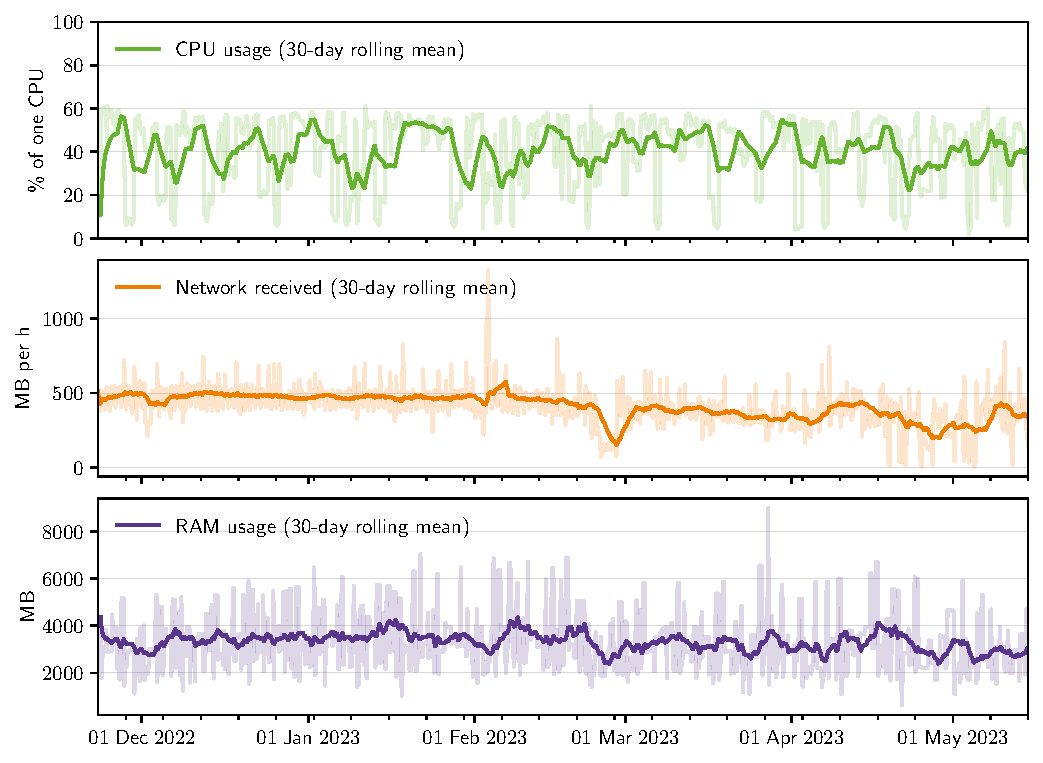
\includegraphics[width=\linewidth]{images/monitoring-prediction-service-load.pdf}
    \caption{Cadvisor statistics for prediction service.}\label{fig:monitoring-prediction-service-load}
\end{figure}

Based on collected Cadvisor\footnote{\url{https://github.com/google/cadvisor}} metrics on CPU load, RAM usage, and network load, the prediction algorithm scaled well to the multiple thousand traffic lights. The algorithm was implemented in a Java service that also controlled receiving Observations and sending Predictions to our prediction MQTT broker. We measured the service on a TU Dresden Enterprise VM with 6 CPU cores. To calculate the percentage utilization of the prediction service on the CPU cores, CPU time was measured. In this context, the service consumes approximately 60\% of the CPU time of a single CPU, translating to around 10\% of the total possible computing capacity when considering the 6 CPUs that were available on our VM. Both network usage and RAM consumption also remained within acceptable limits. 

\begin{figure}[t]
    \centering
    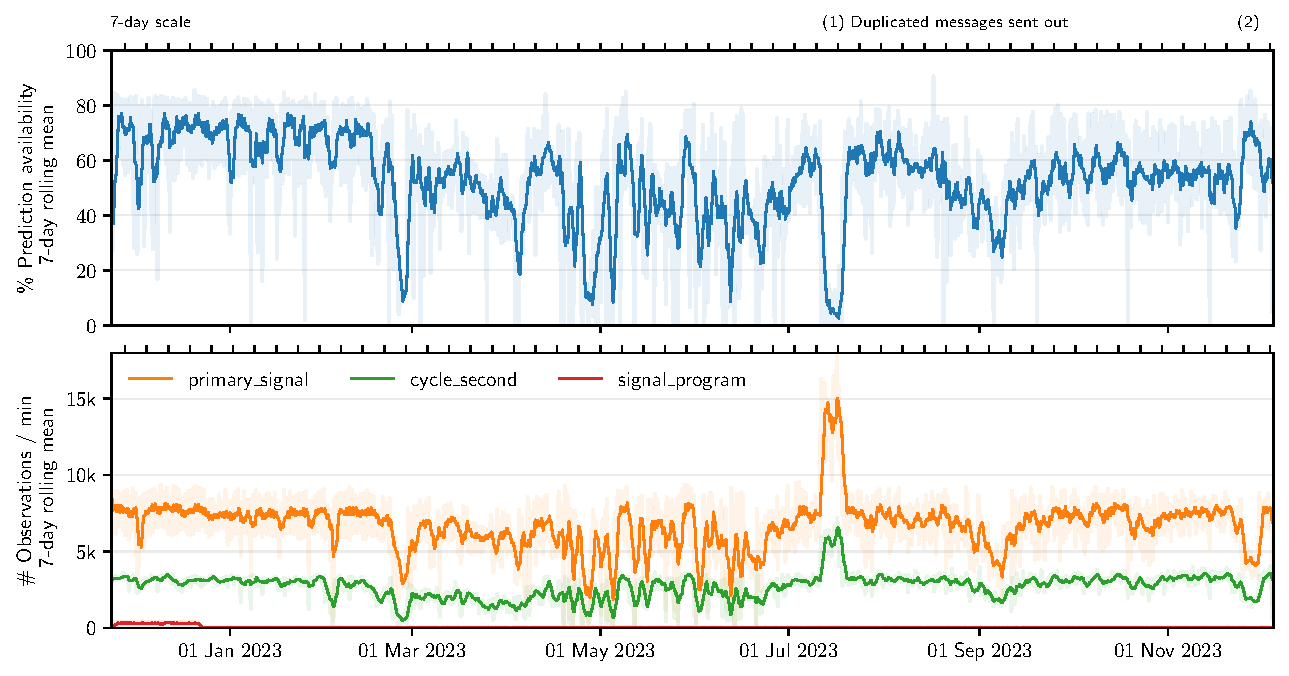
\includegraphics[width=\linewidth]{images/monitoring-availability.pdf}
    \caption{Long-term development of prediction availability.}\label{fig:monitoring-availability}
\end{figure}


The long-term data trend and prediction availability are depicted in \Cref{fig:monitoring-availability}. The prediction availability is calculated by dividing the number of predictions generated per minute by the total number of available traffic lights. In the upper part of the figure, we observe that prediction availability typically fluctuates between 40\% and 80\%, with 100\% never being reached. For the time period given in the diagram, we calculate a median prediction availability of 55.07\% (IQR: 28.23\%). The maximum observed prediction availability resides at 90.63\%, recorded on September 17, 2023, at 0:00. Thus, the median prediction availability is quite low throughout the studied period, while some weeks showed good service availability.

The visible disruptions in prediction availability can be primarily attributed to short-term data errors in the Traffic Lights Data system. For instance, around July 11, 2023 (1), all observations were accidentally sent twice, causing prediction availability to nearly drop to 0\%. Examining the long-term trend, we notice increased disruptions in prediction availability in the summer of 2023, following an initial period of relatively stable availability. These disruptions coincided with increased maintenance activities on the Traffic Lights Data System, indicating that repeated updates during this period led to a deterioration in data quality. 

Although an increase in prediction availability can be seen around November 23, 2023 (2), this increase originated from us excluding erroneous traffic lights from our prediction service, also decreasing the overall number of Observations received. The prediction availability over the period under consideration was, therefore, not optimal.

\begin{figure}[t]
    \centering
    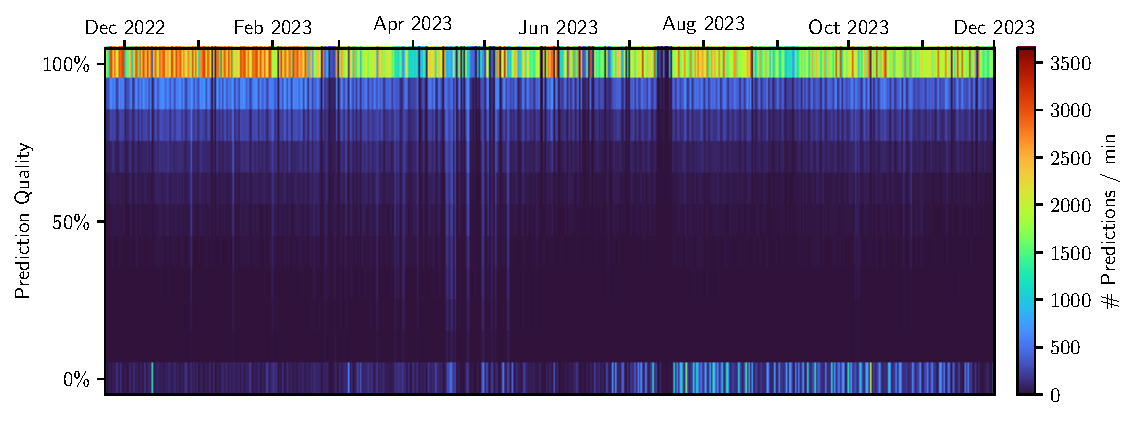
\includegraphics[width=\linewidth]{images/monitoring-long-term-study.pdf}
    \caption{Long-term development of prediction quality.}\label{fig:monitoring-long-term-study}
\end{figure}

In addition to the prediction availability, we also measured the prediction quality through a continuous comparison of the prediction with the actual incoming data. If every second in the prediction vector aligns with the currently running cycle, the prediction quality is calculated as 100\%. If no seconds align, this results in 0\% prediction quality. The running cycle is not incorporated into the prediction vector yet at the time of prediction quality calculation, ensuring that no running information sinks into the calculated prediction quality. In the current implementation of the prediction procedure, there is also a prediction quality of -1, generated when real-time data is no longer available to validate the prediction for an extended period of time. In \Cref{fig:monitoring-long-term-study} that shows the result of this recording, this is mapped as a prediction with 0\% quality.

Considering the 10\% buckets in which the prediction quality was monitored, the calculated median prediction quality resides at 85.78\% (IQR: 1.85\%). Examining the long-term trend initially reveals a similar pattern in prediction availability at 100\% quality compared to \Cref{fig:monitoring-availability}. For example, there was also a significant dip around July 11, 2023, due to the duplicated messages issue and a general decrease in availability throughout the year 2023. In addition, we can see in this diagram that fewer predictions fall within the intermediate 10\% to 90\% quality range. As the increased data outages in summer 2023 coincide with an increase in low-quality predictions, it is likely that most of the predictions below 10\% quality are due to temporarily missing data. Thus, if interpreted as an accuracy metric, many predictions that were generated with consistent traffic light data likely have been precise to a few seconds.

\begin{figure}[t]
    \centering
    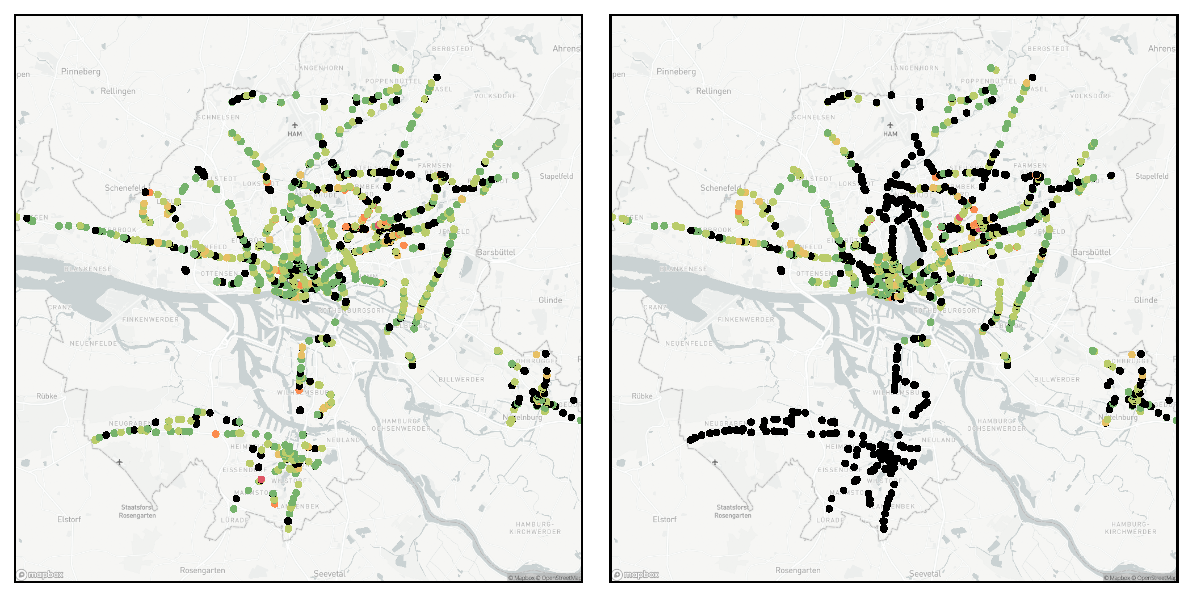
\includegraphics[width=\linewidth]{images/monitoring-before-after-failure.pdf}
    \caption{Before and after traffic controller failure on Oct 11, 2023. [\hyperref[attribution]{Attribution}]}\label{fig:monitoring-before-after-failure}
\end{figure}

The decline in prediction availability observed in the summer of 2023 has had multiple origins, many of which could be identified through our monitoring tools, reported, and ultimately addressed. The first two kinds of data error that could be pinpointed are highlighted in  \Cref{fig:monitoring-before-after-failure}: blackouts of individual traffic lights (on the left and right) and blackouts affecting entire city districts (on the right only).

Through our map-based prediction quality monitoring, we could help identify 61 intersections and 80 individual connections experiencing persistent issues, rendering them unable to transmit data. In at least 30 cases, a connection was falsely associated with an unsignaled road crossing, or the connection was no longer present. Among 22 nodes, traffic lights utilized the OCIT protocol, which is, at the time of writing, unsupported by the Traffic Lights Data platform. For 19 nodes, the observed failures are presumed to be construction-related, with this confirmed in three additional cases. In 16 instances, outdated intersection topologies or georeferences were identified. The identified traffic lights were subsequently excluded from the prediction system using an exclude list, with the option to reintegrate them later.

Turning our attention to failures affecting entire city districts, \Cref{fig:monitoring-failure} demonstrates their relatively spontaneous occurrence. This type of failure poses a more significant challenge than individual intersection or connection failures since thousands of predictions are abruptly invalidated. Therefore, we worked rigorously together with the platform operators to identify the source of this issue.

\begin{figure}[t]
    \centering
    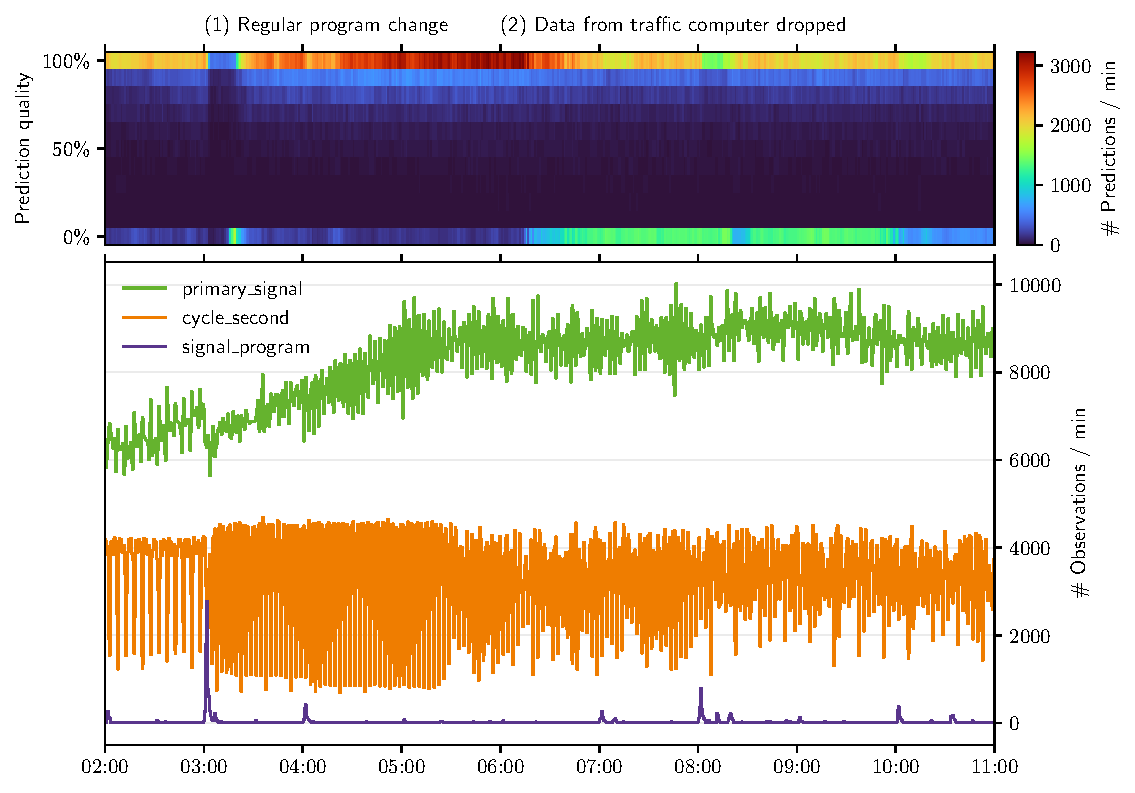
\includegraphics[width=\linewidth]{images/monitoring-failure.pdf}
    \caption{Monitored metrics during traffic controller failure on Oct 11, 2023.}\label{fig:monitoring-failure}
\end{figure}

To better understand the occurrence of such a failure, we examined the daily data course recorded by our monitoring system, as depicted in \Cref{fig:monitoring-failure}. At 3:00 AM UTC, within the timeline of \texttt{signal\_program} Observations, we see that many traffic lights switch their programs. As confirmed by traffic light operators, this pattern represents the morning program of the weekly automation of the traffic lights being scheduled.

Simultaneously, the availability and quality of the predictions briefly decline (1). This can be explained by the fact that the prediction algorithm continues to forecast the old pattern from the previous program for a short period, only synchronizing with the new program after approximately 15 minutes (or 10 cycles at 90 seconds). The reason is that the prediction service continues to record cycles and pushes out older cycles from the prediction window only after a few minutes. One identified solution for this issue is to switch between histories recorded for each traffic light once a program Observation arrives.

Following this brief decline, the best prediction quality is achieved around 6:00 AM UTC, just before it suddenly and persistently collapses across multiple districts. The fact that these declines are reflected in specific districts strongly suggests that this issue can be traced back to specific traffic controllers, each generating Observations for one or more districts. 

Once this finding was communicated to the operators of the Traffic Lights Data platform, it was identified that this problem is indeed associated with certain traffic controllers. The increasing load throughout the day due to rising traffic triggering more green phases causes the message queues of the MQTT brokers at the traffic controllers to fill up. Ultimately, this results in the traffic controllers either not sending messages at all, dropping individual messages, or transmitting them with significant delays.

\begin{figure}[t]
    \centering
    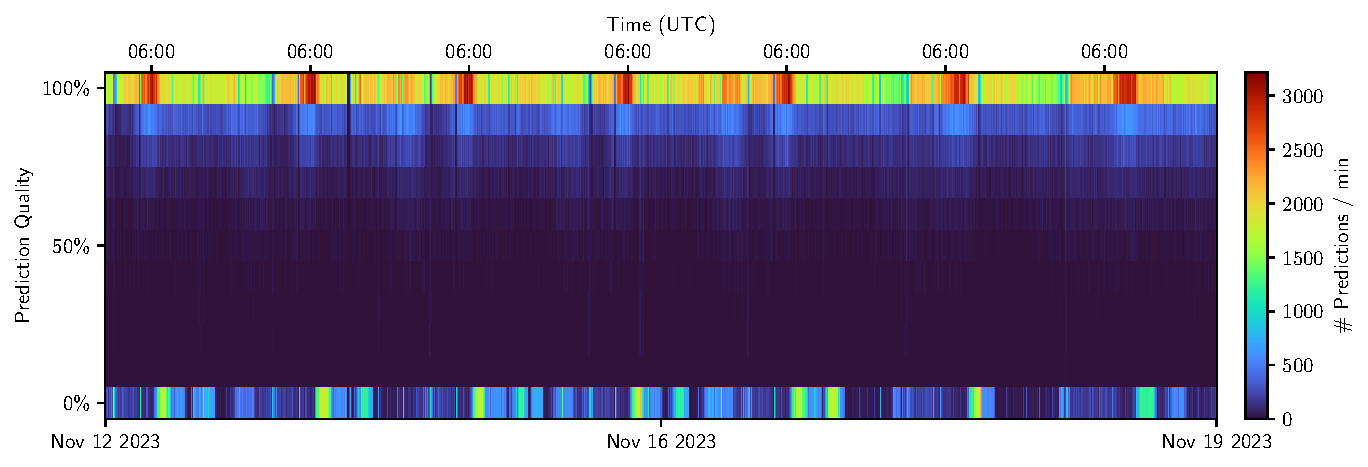
\includegraphics[width=\linewidth]{images/monitoring-7-days.pdf}
    \caption{Reoccurring traffic controller failures after 6:00 UTC.}\label{fig:monitoring-7-days}
\end{figure}

In the weekly progression illustrated in \Cref{fig:monitoring-7-days}, it becomes evident that this situation repeated almost daily at the same time. Only on Saturdays and Sundays does the issue manifest later, around 7:00 -- 8:00 AM UTC, due to reduced and delayed traffic leading to fewer green phases.

Upon identifying the root cause, the operators initiated appropriate fixes related to the MQTT queues of the traffic controllers. Simultaneously, we created an additional exclusion list of intersection nodes, preliminarily exempting them from the prediction until the issue was resolved. This involved a total of 584 intersections connected to three specific traffic controllers. Due to compliance concerns, the operators have not allowed us to disclose the specific traffic controllers that were affected; however, further information in this regard can be found in a technical report from 2020 \cite{neuner_leitfaden_2020}. 

Looking at the number of discarded cycles, we derive further insights into whether isolated messages are lost or if observations from operational traffic lights consistently reach their destination. The analysis is depicted in \Cref{fig:monitoring-rejected-cycles} and started around August 1, 2023. Here, after a longer period with invalid cycles, we see a substantial improvement around October 31 at 6:40 AM local time. The number of rejected cycles suddenly dropped to 0, with only sporadic peaks. This indicates that another data issue in the Traffic Lights Data platform was addressed; however, we could not trace back which specific modification was made at that time. Before, between 25 and 125 cycles were rejected every minute, indicating that the issue could have affected up to 200 connections throughout summer 2023, assuming a cycle length of 90 seconds. 

After identifying issues with the traffic controllers and falsely importing traffic lights in the data platform, we were also able to identify issues related to the router installed at the platform operator's servers, which was not able to keep up with all messages. The corresponding router was replaced, further improving the data quality. The stability of the MQTT brokers that were directly connected with the traffic controllers was also optimized by scaling up the computational resources of the virtual machines that were handling the message exporting. As a result of these efforts, the original prediction availability from 2022 (80\% during the day) could be restored in February 2024, stabilizing the Traffic Lights Data system.

\begin{figure}[t]
    \centering
    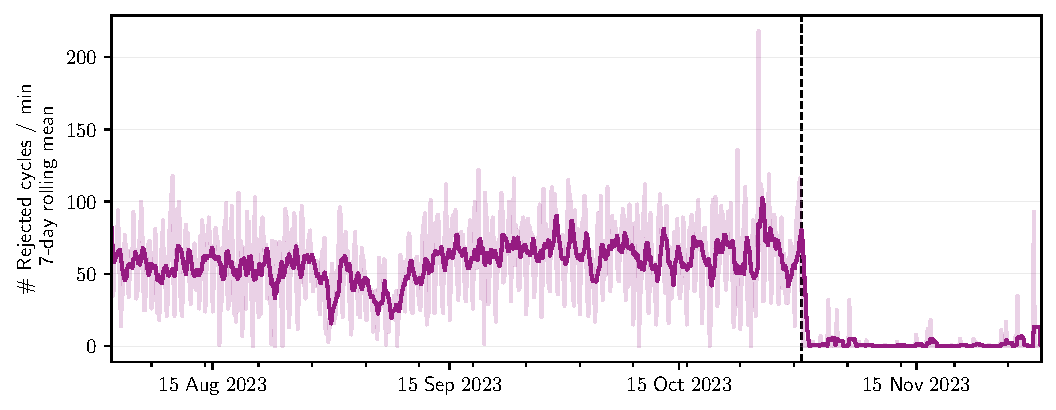
\includegraphics[width=\linewidth]{images/monitoring-rejected-cycles.pdf}
    \caption{Cycles rejected due to out-of-order phase sequence.}\label{fig:monitoring-rejected-cycles}
\end{figure}

\subsection{Study of Traffic Light Predictability in Hamburg}

In the previous section, we found that the prediction availability for traffic lights in Hamburg was low during 2023, but the main part of this issue could be attributed to data issues. The prediction quality was also likely affected by data issues, as predictions would be invalidated by the missing data, resulting in a prediction quality of -1 (no validation possible) that was mapped to 0\% in the monitoring. We found that the remaining predictions were mostly centered on 90\% to 100\% quality, more than we expected with the high prevalence of adaptivity-capable traffic lights in Hamburg. This finding was also one of the key motivations for us to further investigate the overall predictability of traffic light patterns. 

To conduct these evaluations, real-time data was recorded for four weeks. This encompassed 19,844 individual traffic lights available in the Traffic Lights Data system at the time of evaluation, including all modes of transport and not only cyclist traffic lights, as in the previous study. During the measurement period, data was obtained from 18,009 (90.75\%) of all traffic lights, among which 519 traffic lights also contained secondary signal data. Thus, although we implemented supplementation of the MQTT messages over the Traffic Lights Data platform's HTTP interface, there were some traffic lights that never sent data.

Nonetheless, the supplementation was still effective in addressing partial data outages, as seen in \Cref{fig:adaptiveness-mqtt-http}. On multiple days, approximately half of all recorded observations were supplemented by the HTTP interface because they were lost preliminarily via MQTT. However, a minor dip in messages remained for some days, meaning that small parts of the messages could not be recovered.


\begin{figure}[t]
    \centering
    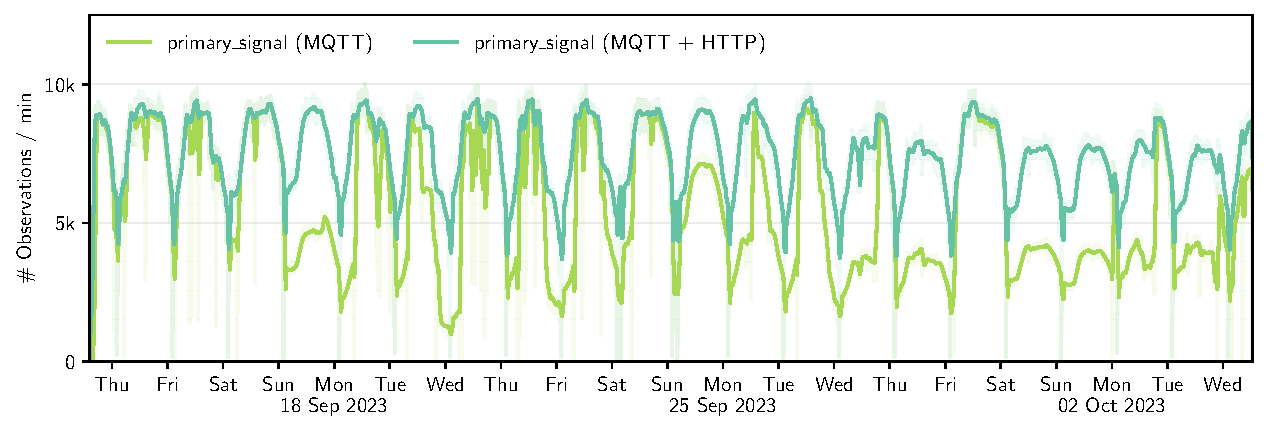
\includegraphics[width=\linewidth]{images/adaptiveness-mqtt-http.pdf}
    \caption{Supplementation of recorded MQTT observations through HTTP interface.}\label{fig:adaptiveness-mqtt-http}
\end{figure}


The detection of faulty cycles, also implemented in the prediction service, was utilized for problem identification. Out of approximately 424 million reconstructed cycles, 13.8 million cycles were discarded. Here, 90\% of faulty cycles are distributed across 10\% of the connections. By examining the faulty connections on the map, one of the known faulty traffic controllers could be identified as the main cause. These numbers are related to the 40\% of traffic lights that were detected to switch between green, (red-)amber, and red. 34\% of traffic lights that only switched between green and red could also have generated erroneous cycles that were not discarded. The remaining 26\% of traffic lights are comprised of a large variety of other switching patterns. The 2106 traffic lights for which an error rate of >10\% was detected were excluded from further analyses.

\begin{figure}[!t]
    \centering
    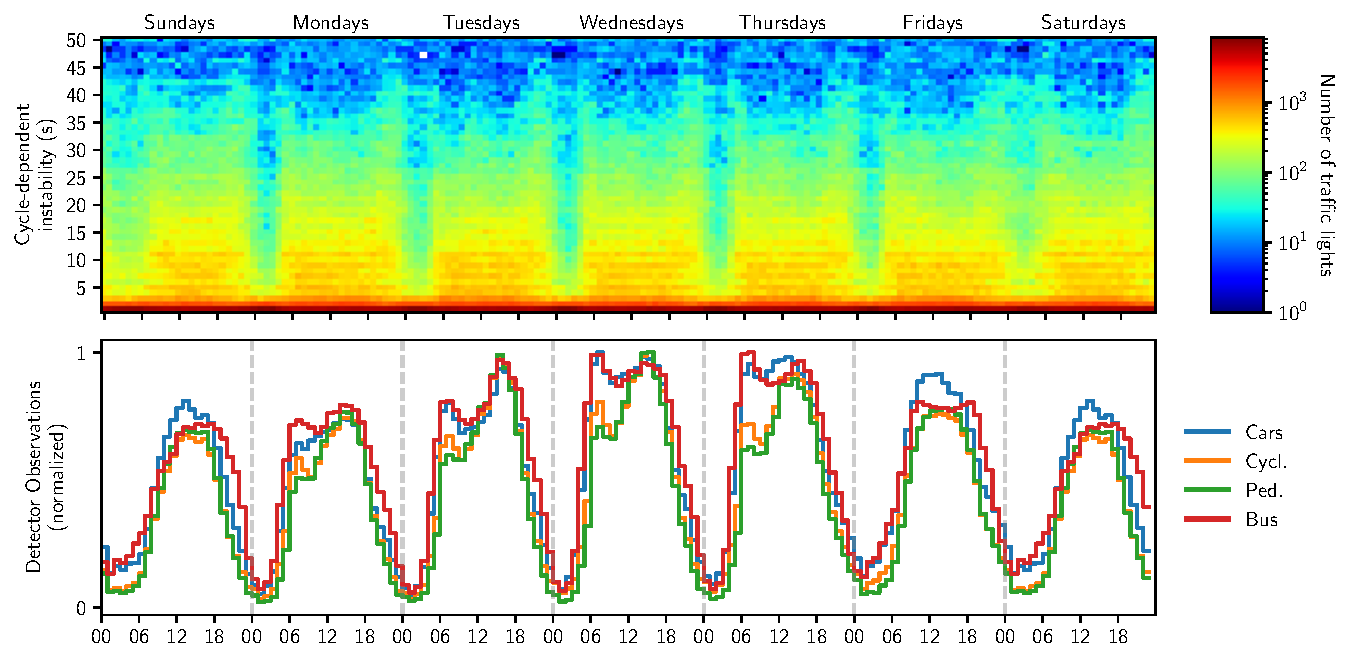
\includegraphics[width=\linewidth]{images/predictability-week-heatmap.pdf}
    \caption{Measured traffic light instability over weekdays in relation to the measured traffic volume.}\label{fig:adaptiveness-weekdays-distance}
\end{figure}

Thus, we could not completely eliminate all errors, but they seem to be present only to a minor extent. We assume that isolated recording errors are overshadowed by the mass of valid data. However, it is important to note for subsequent analyses that recording errors may have occurred, e.g., missing cycle observations leading to multiplied cycle lengths. Accordingly, we will use statistics for evaluation that are robust to outliers.

The first chart displayed in \Cref{fig:adaptiveness-weekdays-distance} looks at the relation between traffic light predictability and daytime. As a statistically robust measure against outliers in the data, we use the median of the cycle discrepancy and wait time diversity for all recorded hourly buckets to analyze how unpredictability evolves during the day. The information is presented along with the frequencies of recorded traffic detector Observations to compare the measured predictability to the measured traffic volume.

As a result, we observe that predictability decreases, as expected, with increasing traffic volume. While the predictability is at its highest during the night, it declines rapidly during the morning traffic surge. However, it then remains relatively constant after reaching a lower bound until the evening before increasing again. The relatively constant predictability during daytime indicates that there may be limits to the adaptiveness even in the presence of increasing traffic. 

Another finding is that most traffic lights were measured with low cycle discrepancy and wait time diversity values, even throughout the day, by one order of magnitude. Measured across all traffic lights, the median cycle discrepancy ranges between 0 and 2 seconds depending on the daytime. The highest median cycle discrepancy during the day comprises only 10\% of the median green length that is measured at 20 to 23 seconds during these times, meaning that green phases largely overlap between cycles. The wait time diversity shows a similar pattern, although the number of traffic lights with 100\% increases during nighttime. The reason for this increase is likely that traffic lights switch to fewer green phases, increasing the chance that the waiting time between green phases is unique.

\begin{figure}[t]
\centering 
\begin{tabular}{@{}cc@{}}
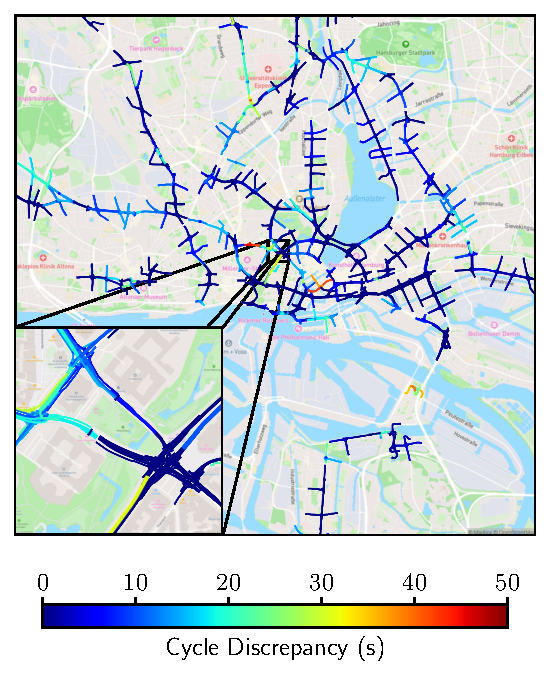
\includegraphics[width=0.46\linewidth]{images/predictability-map.pdf} & 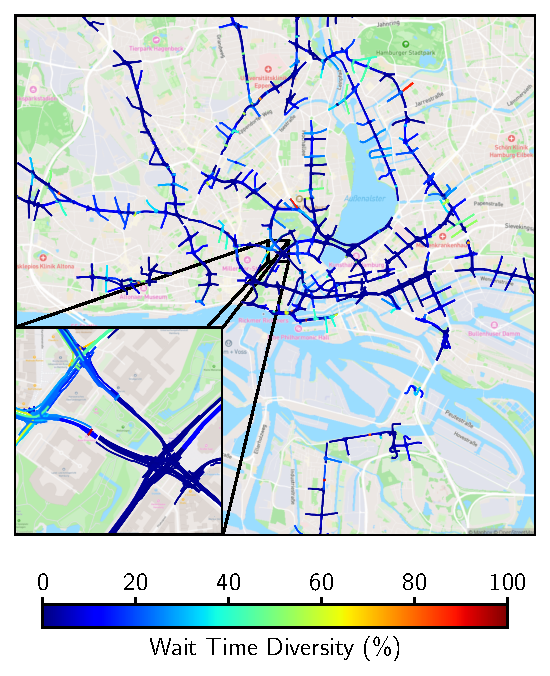
\includegraphics[width=0.46\linewidth]{images/predictability-map-diversity.pdf}
\end{tabular}
\caption{Spatial distribution of predictability. [\hyperref[attribution]{Attribution}]}\label{fig:predictability-map}
\end{figure}

\Cref{fig:predictability-map} shows how our predictability metrics are spatially distributed across intersections in Hamburg. While the majority of traffic lights in both images are located in the blue range of the color scale, indicating a high level of predictability, there are indeed traffic lights where a higher cycle discrepancy or wait time diversity can be observed. 

As expected, traffic lights with higher unpredictability seem to be located together at the same intersection since they share a common program and depend on each other's ingress directions. This can be seen in the zoomed-in part of the diagram. However, it can also be seen that in many cases, traffic lights only exhibit one kind of unpredictability and not both. Traffic lights exhibiting both unpredictabilities seem to be quite rare.

\begin{figure}[!t]
    \centering
    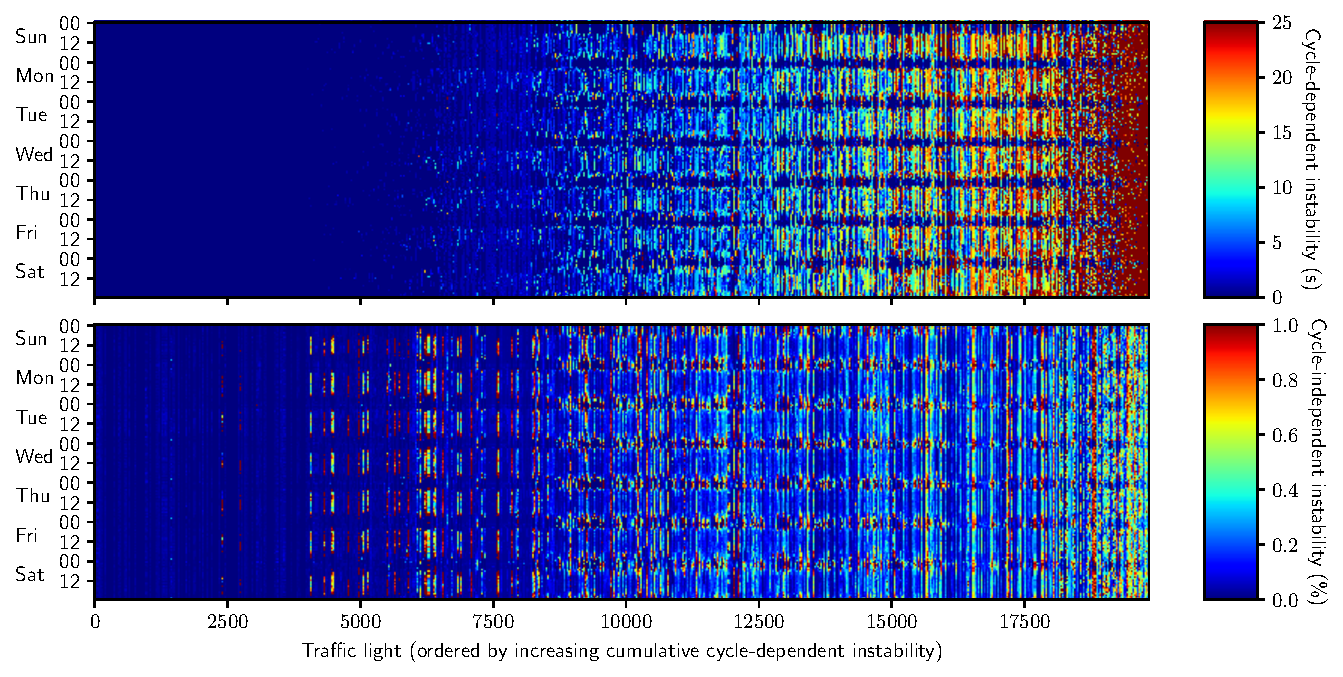
\includegraphics[width=\linewidth]{images/predictability-week-heatmap-per-thing.pdf}
    \caption{Weekly progression of both predictability metrics for each traffic light, represented by a vertical line each.}\label{fig:predictability-week-heatmap-per-thing}
\end{figure}

This aspect is explored further in \Cref{fig:predictability-week-heatmap-per-thing}. In the leftmost part of the diagram, traffic lights can be seen that have a low cycle discrepancy but express a high wait time diversity. In the rightmost part, there are also traffic lights with high cycle discrepancy that express low wait time diversity. For these traffic lights, our chosen prediction method may not be ideal. 

Out of the evaluated 2,793,786 traffic light hours, 43\% (1,206,817) have a cycle discrepancy of less than 5 seconds and a wait time diversity of less than 10\%. For 67\% of traffic light hours, a cycle discrepancy lower than 5 seconds could be measured, which may also contain higher wait time diversities. Only regarding wait time diversity, 77\% of recorded traffic light hours reside below 20\%. Hardly predictable traffic light hours, meaning that the wait time diversity is above 20\% and the cycle discrepancy is above 5 seconds, only comprise 12\% of the overall dataset. Note that the 5-second cycle discrepancy and 20\% wait time diversity were chosen here somewhat arbitrarily as a decision boundary, which we felt constituted a good predictability for our scenario. The decision boundary may be chosen more loosely or also strictly, depending on the requirements. Nonetheless, the tendency is clear that a large proportion of traffic lights fall into a high predictability region. 

\begin{figure}[t]
    \centering
    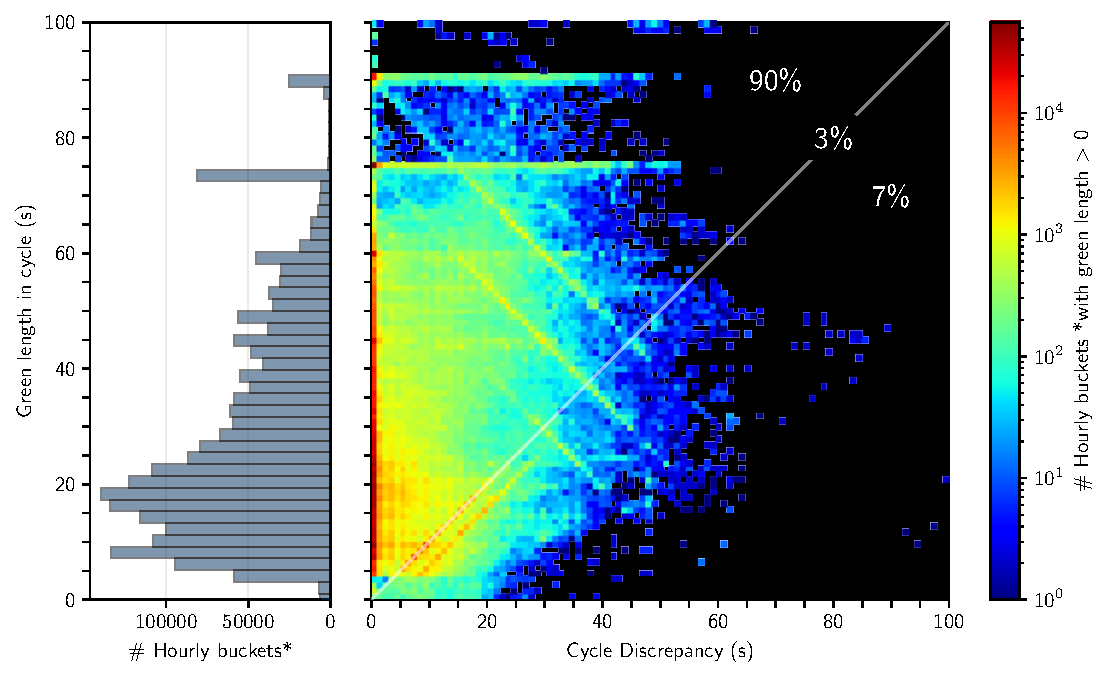
\includegraphics[width=\linewidth]{images/cycle_discrepancy_green_length_heatmap.pdf}
    \caption{Green length and cycle discrepancy.}\label{fig:green-length-cycle-discrepancy}
\end{figure}

The results must be seen in correspondence to the measured green length, which determines how much green overlaps between cycles. A high green overlap, even in the presence of a high cycle discrepancy, would mean that our probabilistic prediction method still finds safely green regions that are suitable for speed advisory. As seen in \Cref{fig:green-length-cycle-discrepancy} for 90\% of recorded traffic light hours, the median green phase is longer than the median cycle discrepancy. What should be noted here, again, is that most of the traffic light hours reside all the way to the left at a cycle discrepancy of zero seconds.

Interestingly, there are also some patterns that allow us to further understand the constraints in traffic light behavior. First, a clear cutoff at 5 seconds of green length can be seen, which is also prescribed by German traffic light planning \cite{TN_libero_mab2}. When extracting and analyzing random examples from specific regions, we find that the horizontal concentrations at 90 seconds, 75 seconds, and 60 seconds primarily stem from traffic lights that switch green for the complete cycle. These buckets are occasionally shifted to the right by red phases of different lengths that interrupt the otherwise switched green phase. Top-left to bottom-right diagonal lines seem to come from traffic lights that extend their green phase until a maximum green duration is reached. Since shorter green phases can be placed more flexibly in the cycle, a decreased green length leads to a higher cycle discrepancy. These constraints could be detected and used to improve the prediction.

\begin{figure}[t]
    \centering
    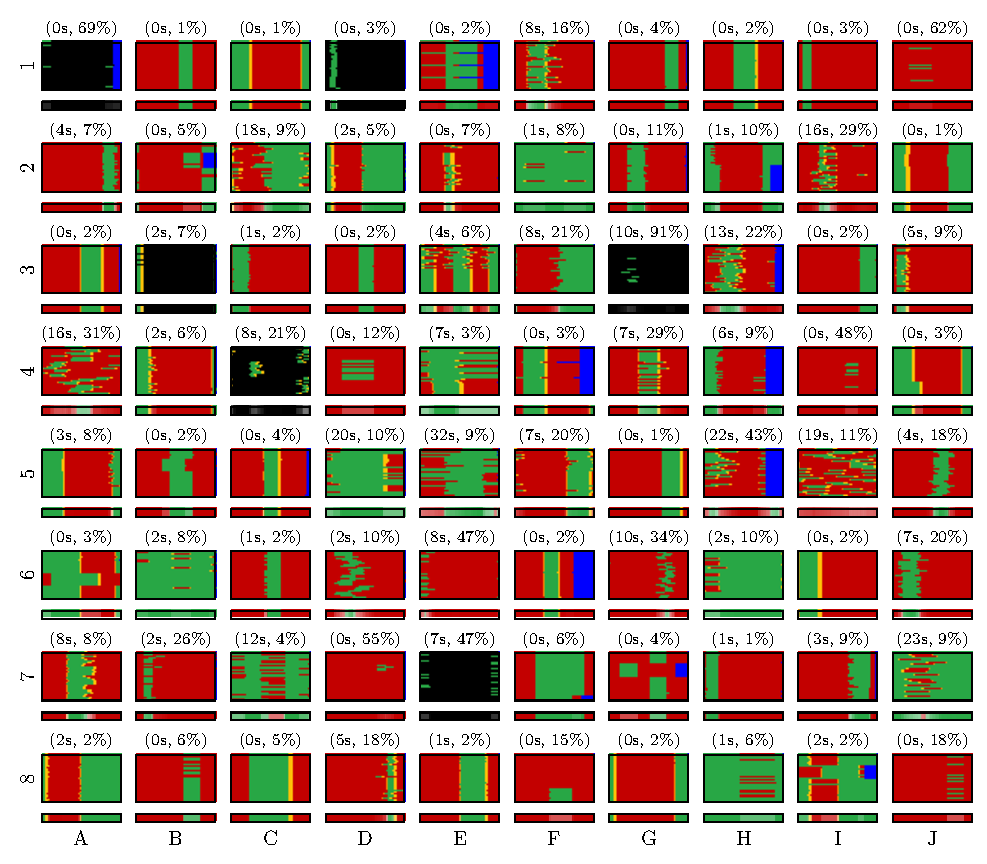
\includegraphics[width=\linewidth]{images/predictability-case-studies.pdf}
    \caption{Examples of recorded traffic light histories, ordered by their classification according to our two metrics. Below each cycle diagram, a probabilistic prediction based on the cycles is shown. Title format: median (cycle discrepancy, wait time diversity).}\label{fig:types-of-instability}
\end{figure}

So far, we have considered abstract measures of predictability to obtain an overall understanding of how many traffic lights are hard to predict. To conclude this study, we validate our findings through a random sample of traffic light hours that were extracted from the recorded database. The extracted sample is highlighted in \Cref{fig:types-of-instability} together with the associated values for cycle discrepancy and wait time diversity. Predictions are also shown that incorporate all cycles in the recorded bucket, to demonstrate how a probabilistic prediction displayed to the user would look like. As seen in the visualization, the sample also contains traffic lights that switch between green and black, as well as samples in which the cycle length changed in between, indicated by the blue background.

Overall, most recorded buckets in this sample contain behavior that can be considered predictable. Only in the first row, there are already 6 out of 10 cases (B1, C1, E1, G1, H1, I1) in which there are clear columns in the switching pattern, that can be easily predicted. There are also cases such as D1, A2, D2, or G2, in which an adaption is clearly visible but limited to a few seconds. In examples such as F2, D5, or H8, we can see traffic lights that are always green until disrupted by a red phase. For cases such as C2, E3, H3, A7, or J7, the traffic adaptivity is clearly more pronounced, as also reflected by the high cycle discrepancy score. However, in these cases, as seen before, a common part in which all cycles are green can still be identified. This is not the case for examples such as D6 or G6, while these examples also indicate that the green phase centers around a midpoint, as shown in the prediction. A completely unpredictable pattern seems to be given in I5. Here, the prediction is fully blurred out. With G7, we also find one example in which the program seems to have been switched out, indicated by the sudden change in the otherwise stable pattern. Finally, we also see switching behaviors such as E6, J1, J8, or D7, in which the traffic light is switched red most of the time, leading to a red prediction.

In general, while there are examples in which a clear adaptive behavior can be seen, most recorded switching behaviors contain predictable patterns. This can also be seen by the probabilistic prediction below each cycle diagram, which is only blurred out marginally for most predictions. Most predictions contain at least a small fraction of each green phase that is certain. Thus, our case study, while highlighting a few interesting examples, generally confirms our previous findings.

\begin{Summary}[Summary and Discussion of Results]
Our results clearly show that we cannot assume from centralized traffic light data systems that they deliver stable and consistent data. In our case, long-term collaboration with platform operators and active error searching were necessary to ultimately stabilize the data system. Previous studies may have been too optimistic here, especially studies that don’t work with a real-world system. The highly federated architecture in such systems may lead to complex failure patterns that must be accounted for in the prediction algorithm. 

Through the developed monitoring system, we could identify and help fix multiple systematic issues in Hamburg’s Traffic Lights Data infrastructure, taking over a key part of the urgently needed quality assurance process. In particular, we could determine a failure pattern related to the traffic controllers that reoccurred daily, helping the operators to scale the data brokers accordingly. Multiple other issues at various parts of the data platform's pipeline were also found and could ultimately be identified and fixed. Even in the presence of these harsh circumstances, the probabilistic approach seemed to scale well and showed good accuracy at most intersections, while the prediction availability was often not optimal due to the described data outages.

Then, we looked at the general predictability of traffic lights in a broader perspective. We found that the predictability decreases during the day together with the traffic surge, but not as much as expected. We measured that traffic lights seem to indeed switch more adaptive and thus unpredictable during daytime. However, the traffic adaptation seems to be highly limited for most traffic lights, as the predictability only decreases to a limited extent, while a large proportion of traffic lights stay entirely unaffected. 

Thus, compared to the 90.7\% of traffic lights in Hamburg that should be able to adapt to traffic conditions, we find that this adaptation is only minorly expressed, if at all. Most observed switching patterns align with the cycle length, meaning that the probabilistic approach, which highly depends on this alignment is overall a good choice. If shifts of the phases in cycles are seen, they are usually shorter than the green time, meaning that some parts of the green phases overlap, allowing our method to predict certainly green parts of the traffic light switching behavior. This was also seen in our randomized case study. Nonetheless, a few intersections were seen at which future experimentation with other methods may be indicated.
\end{Summary}

\section{Conclusions}

Traffic light prediction provides many opportunities for future intelligent transport systems to enhance the efficiency and safety of traffic, overcoming issues like dilemma zones when approaching an intersection. In practice, however, traffic light prediction is hindered by two issues: obtaining the traffic light data and accounting for unpredictabilities in the traffic light timing. 

Previous works mainly resorted to DSRC or cellular V2X to obtain traffic light timing information directly. These systems can make use of the residual time that is provided in SPaT messages, externalizing the prediction to the infrastructure provider and ensuring high interoperability between cities. However, as an alternative, we can also use a centralized data platform accessible through the internet, making it widely available to all devices that have access to the cellular network. In general, this solution seems more attractive from a smartphone application's viewpoint. In Hamburg, such a system is available through the Traffic Lights Data platform.

As the Traffic Lights Data platform does not provide traffic light predictions itself, we needed to deploy our own prediction algorithm based on the available real-time data. To achieve this, we looked at prediction algorithms and which ones are accurate, scalable, and resilient to data outages. A probabilistic approach was identified and integrated based on the available data. To cope with data issues, error detection was employed that discards erroneous data and degrades the prediction availability in favor of generating fewer false predictions. 

Based on the calculated prediction quality, the developed prediction system appears to work well at most intersections and fulfill our desired capabilities. Only the availability seems to be an issue induced by the frequent data problems. Through a developed monitoring infrastructure, we could help Hamburg's data broker system operators identify reoccurring failures and plan appropriate fixes. From this process, one key conclusion is that employing a centralized traffic light data system may require large and continued efforts for data quality assurance. We found our monitoring tool a key solution, without which likely fewer issues would have been detected and fixed.

That our prediction algorithm seems to generally work well stands in contrast to previous works that have repeatedly emphasized the problem of traffic adaptivity. Especially in Hamburg, for which a proportion of 95\% adaptive traffic lights was reported \cite{bodenheimer_enabling_2014} and 90.7\% found based on our research, we expected larger problems with negative impacts of traffic adaptivity on our prediction accuracy. Thus, we found a discrepancy between the reported numbers of adaptivity-capable traffic lights and their predictability. To further investigate this discrepancy, we spanned a measurement of two unpredictability metrics across Hamburg for four weeks: wait time diversity and cycle discrepancy. The measurements support our finding that only a few traffic lights express adaptivity to a problematic extent for accurate prediction. Most traffic lights express minor shifts, and green phases are often aligned. A few intersections may impose challenges to our chosen prediction algorithm, indicating the need for experimentation with other prediction methods.

Although the established prediction system can be considered a sound foundation for our bike-GLOSA system that circumvented many issues and contributed to the overall understanding of real-world traffic light predictability, there are also open questions for future work. One issue is a lack of ground truth for traffic light messages. Currently, we have to trust that the traffic light messages contain the correct timing and state information. Traffic lights sending false timestamps can be a real problem, potentially resulting in a certain prediction that does not reflect the real-world situation. To address this issue, we could think of inferring traffic lights sending invalid data, for example, from user trajectories. Even in the presence of minor adaptivity, there could be situations in which the speed advisory is false, requiring users always to pay attention themselves. Calculating probabilities for each second in the prediction is one step in the right direction, ensuring higher trustworthiness and less fluctuation in the speed advisory. However, there are many more steps to go until a prediction can be considered 100\% trustworthy. To reach such a goal, a more direct collaboration between the prediction system and the internal program switching in traffic lights is needed, and a history-based prediction may not suffice.

What was not considered is how we can deploy an advanced prediction model, such as a Machine Learning model, at the intersections that expressed low predictability and whether these models would be able to generate a more accurate prediction, considering that bad predictability often arises from erroneous data. The resilience of these models against these issues should be studied. Optimizing the tradeoff between error robustness, scalability, and fluctuation of the prediction is crucial, not only its accuracy. Future work should focus on this relation to determine under which conditions which model is the most practical.
